\documentclass[letter,12pt]{article}
\usepackage[left=2cm, right=2cm, top=2cm, bottom=2cm]{geometry}
\usepackage[shortlabels]{enumitem}
\usepackage{graphicx}
\usepackage{amsmath}
\usepackage[titletoc,title]{appendix}
\usepackage{amssymb}
\usepackage{makecell}
\usepackage{wrapfig}
\usepackage{verbatim}
\usepackage{listings}
\usepackage{minted}
\usepackage{subfig}
\usepackage{titling}
\usepackage[compatibility=false]{caption}
\usepackage[parfill]{parskip}
\setlength{\droptitle}{1cm}
\usepackage{hyperref}
\hypersetup{
    colorlinks,
    citecolor=black,
    filecolor=black,
    linkcolor=black,
    urlcolor=black
}
\usepackage{setspace}
\renewcommand{\topfraction}{0.85}
\renewcommand{\textfraction}{0.1}
\renewcommand{\floatpagefraction}{0.75}
\usepackage[
    %backend=biber, 
    natbib=true,
    style=numeric,
    sorting=none,
]{biblatex}
\addbibresource{citations.bib}

\setcounter{biburllcpenalty}{7000}
\setcounter{biburlucpenalty}{8000}

\newenvironment{tight_enumerate}{
\begin{enumerate}
  \setlength{\itemsep}{0pt}
  \setlength{\parskip}{0pt}
}{\end{enumerate}}

\newenvironment{tight_itemize}{
\begin{itemize}
  \setlength{\itemsep}{0pt}
  \setlength{\parskip}{0pt}
}{\end{itemize}}

\newlength{\mintednumbersep}
\AtBeginDocument{%
  \sbox0{\tiny00}%
  \setlength\mintednumbersep{8pt}%
  \addtolength\mintednumbersep{-\wd0}%
}

\title{Time-Frequency Representations for Music Source Separation}

\author{\vspace{2em}\\Sevag Hanssian \\
  McGill University \\
 \texttt{sevag.hanssian@mail.mcgill.ca} \\
 \texttt{sevagh@protonmail.com} \\\ \\\ \\
 MUMT 622, Winter 2021 final project\thanks{Source code and materials for this paper are available at \url{https://github.com/sevagh/Music-Separation-TF}}}

\date{}

\begin{document}

\maketitle

\vfill
\clearpage %force a page break

\tableofcontents

\vfill
\clearpage %force a page break

\listoffigures

\listoflistings

\vfill
\clearpage %force a page break



%%%%%%%%%%%%%%
% ABSTRACT			%
%%%%%%%%%%%%%%
\begin{abstract}
	\citet{fitzgerald1} presented an algorithm for separating a musical mix into harmonic and percussive components by masking the short-time Fourier transform (STFT). \citet{driedger} created an iterative version, improving the separation by using two STFTs with different window sizes. \citet{fitzgerald2} replaced the STFT with the constant-Q transform (CQT) to separate vocals. \citet{tfjigsaw}'s Jigsaw Puzzle and \citet{wmdct}'s structured sparsity methods for tonal/transient separation use custom time-frequency analyses based on Gabor expansions and frame theory. This paper presents a survey and evaluation of these different algorithms for harmonic/percussive (and vocal) source separation, from the perspective of the different time-frequency analyses used.
\end{abstract}

%%%%%%%%%%%%%%
% INTRODUCTION		%
%%%%%%%%%%%%%%
\section{Introduction}
\label{sec:intro}

\subsection{Music source separation}

In music analysis (assuming contemporary Western music), important features are driven by the harmonic instruments (e.g., pitch, melody, key), while others (e.g., rhythm, beats, tempo) are influenced more strongly by the percussive instruments. The singing voice contains yet more information, such as the lyrics and song structure. An algorithm for high-quality separation of mixed music into its harmonic, percussive, and vocal components would be generally useful.

The task of music source separation is to split a mixed song into its constituent components, or sources. \citet{musicsepgood} describe that while music source separation could operate on the level of instruments (e.g., saxophone, piano), for simplicity there are broader and more general categories of sources with similar characteristics that can be separated -- harmonic, percussive, and singing voice. In this report, two cases will be considered:

\begin{tight_enumerate}
	\item
		Harmonic/percussive source separation (HPSS) -- also called steady-state/transient separation \cite{bayarres}, or tonal/transient separation \cite{tfjigsaw, wmdct}
	\item
		Harmonic/percussive/vocal (or singing voice) source separation
\end{tight_enumerate}

\subsection{Median-filtering the STFT and CQT}

Harmonic (or steady-state, or tonal) sounds are narrowband and steady in time, while percussive (or transient) sounds are broadband and have a fast decay. \citet{fitzgerald1} noted that they appear as horizontal and vertical lines respectively in the short-time Fourier transform, and applied a median filter in the vertical and horizontal directions to estimate the harmonic and percussive components.

Median filtering is a technique for image processing where a pixel is replaced by the median value of its neighbors in a window, or filter, which slides across all pixels. By applying a median filter shaped like a horizontal rectangle (i.e., stretching in time) to the STFT, vertical (or percussive) features are diminished since their neighboring pixels are empty, preserving horizontal (or harmonic) features. This can be repeated with the axes flipped to obtain the percussive estimate. From these estimates, soft masks are computed which are applied to the original STFT and inverted to create harmonic and percussive signals, shown in figure \ref{fig:fitz1}.

\begin{figure}[ht]
	\centering
	\subfloat[Mixed signal]{{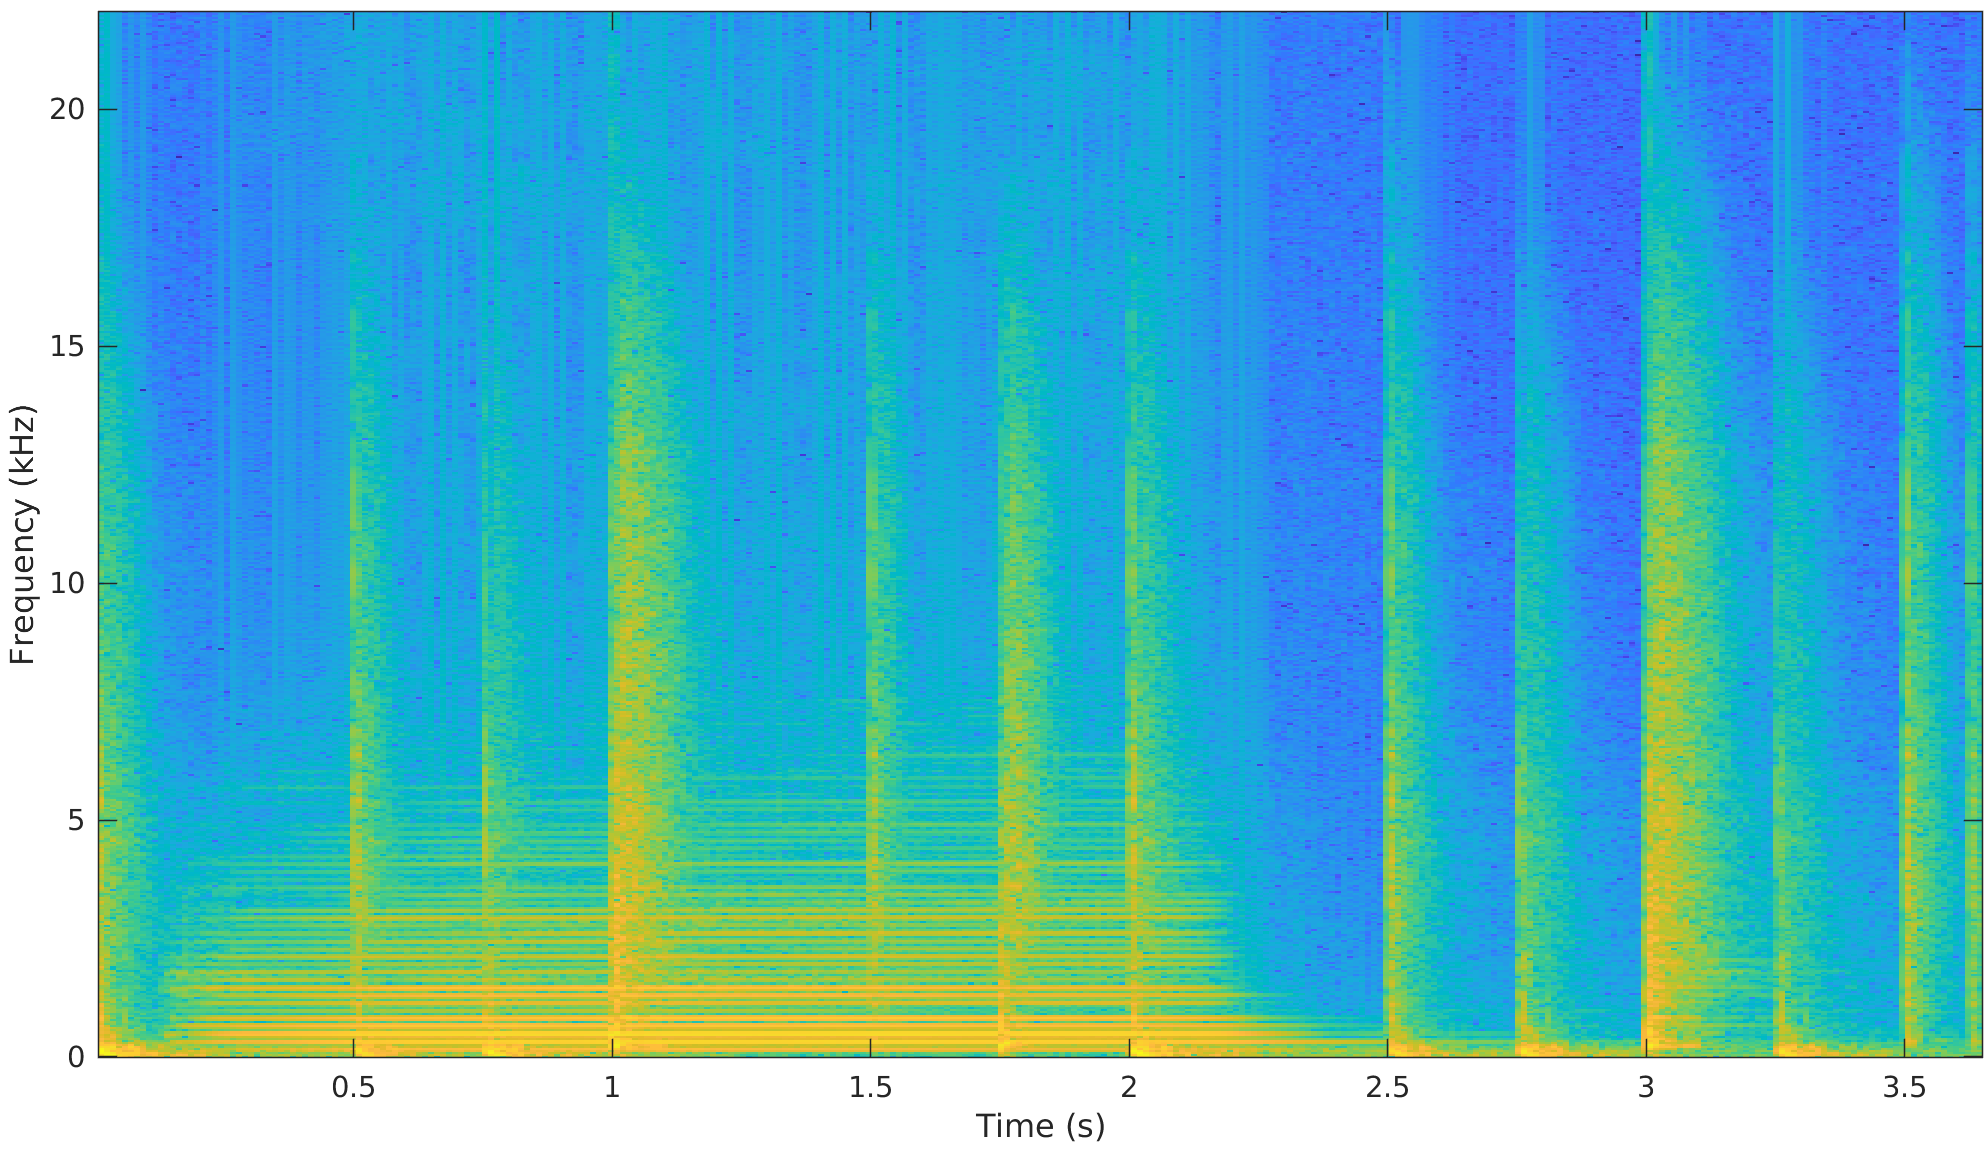
\includegraphics[width=6cm]{./mixedspecgram.png} }}
	\subfloat[Percussive separation]{{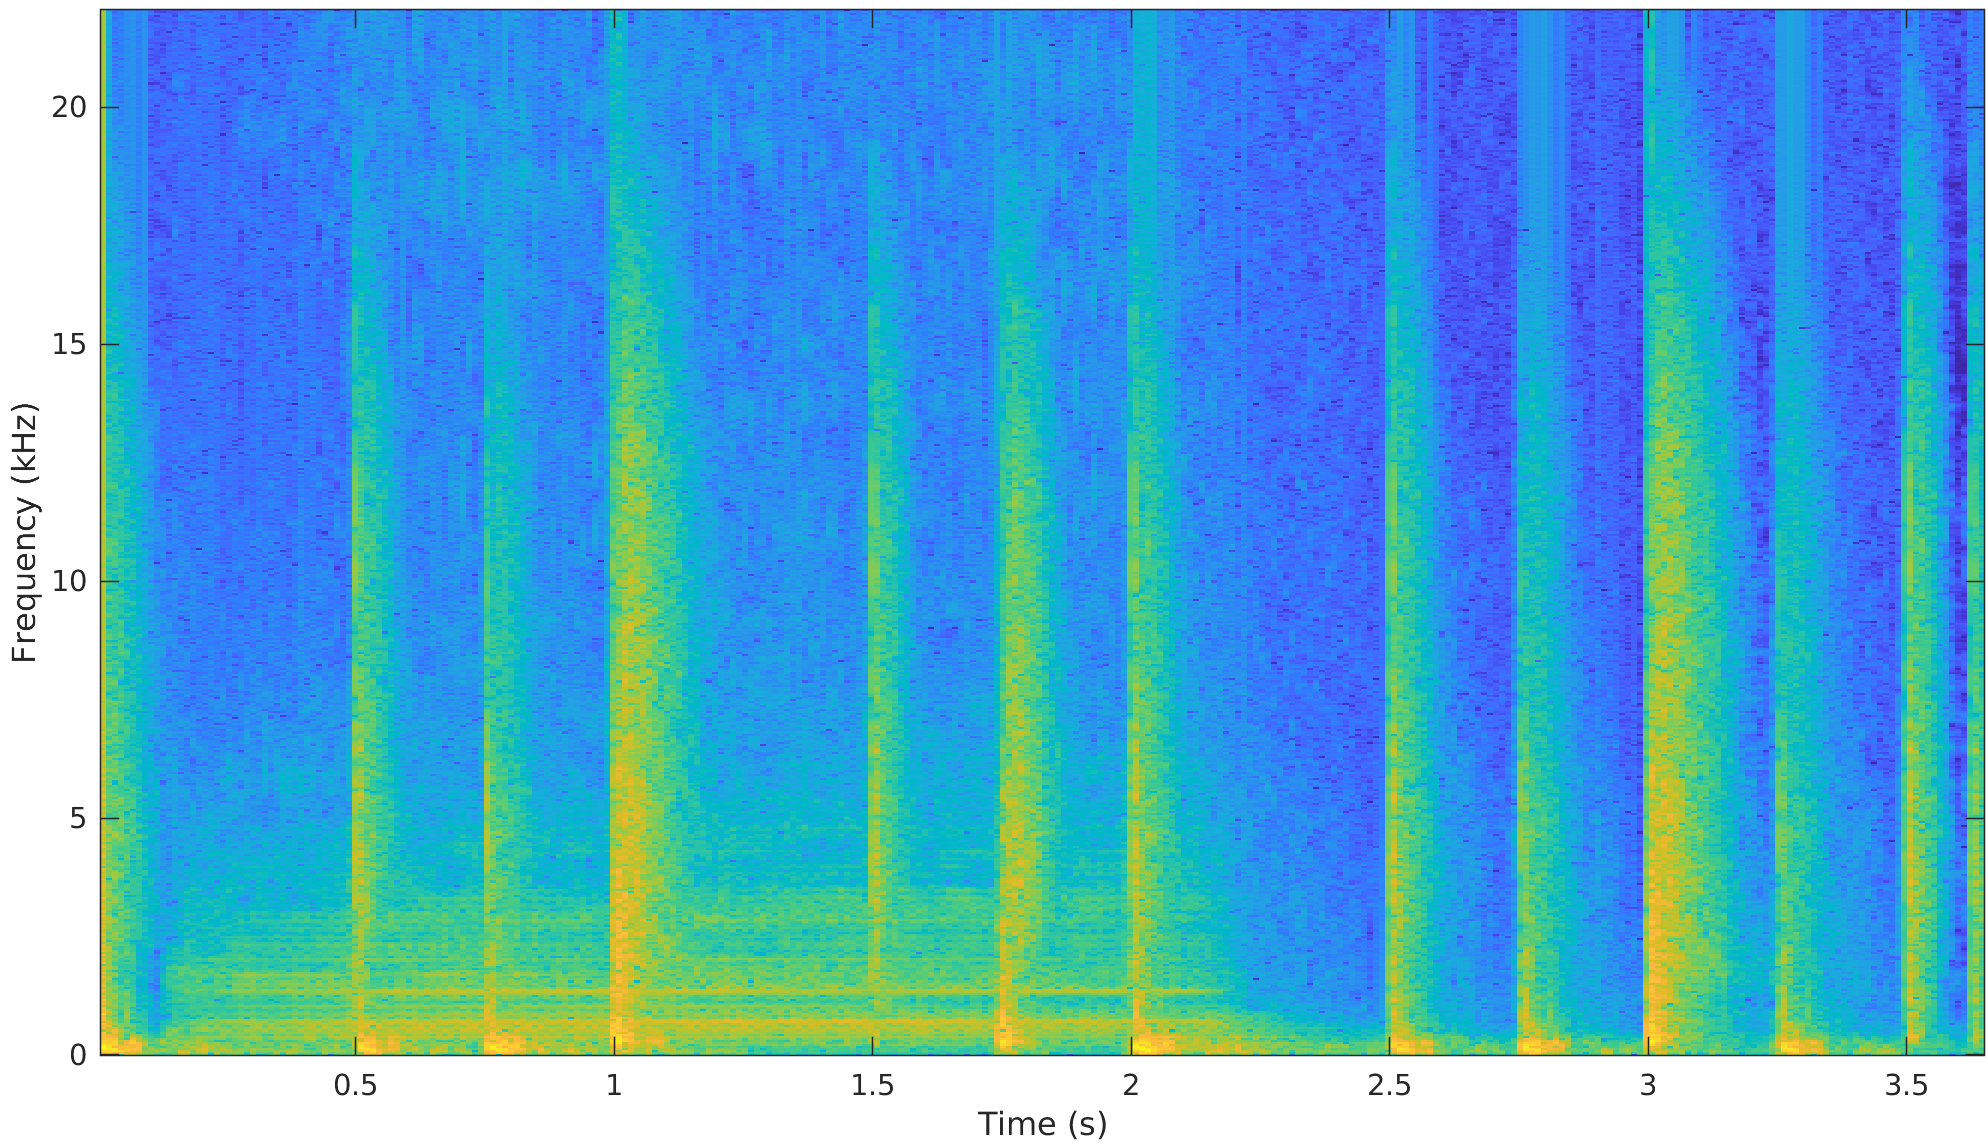
\includegraphics[width=6cm]{./perc_soft.png} }}
	\subfloat[Harmonic separation]{{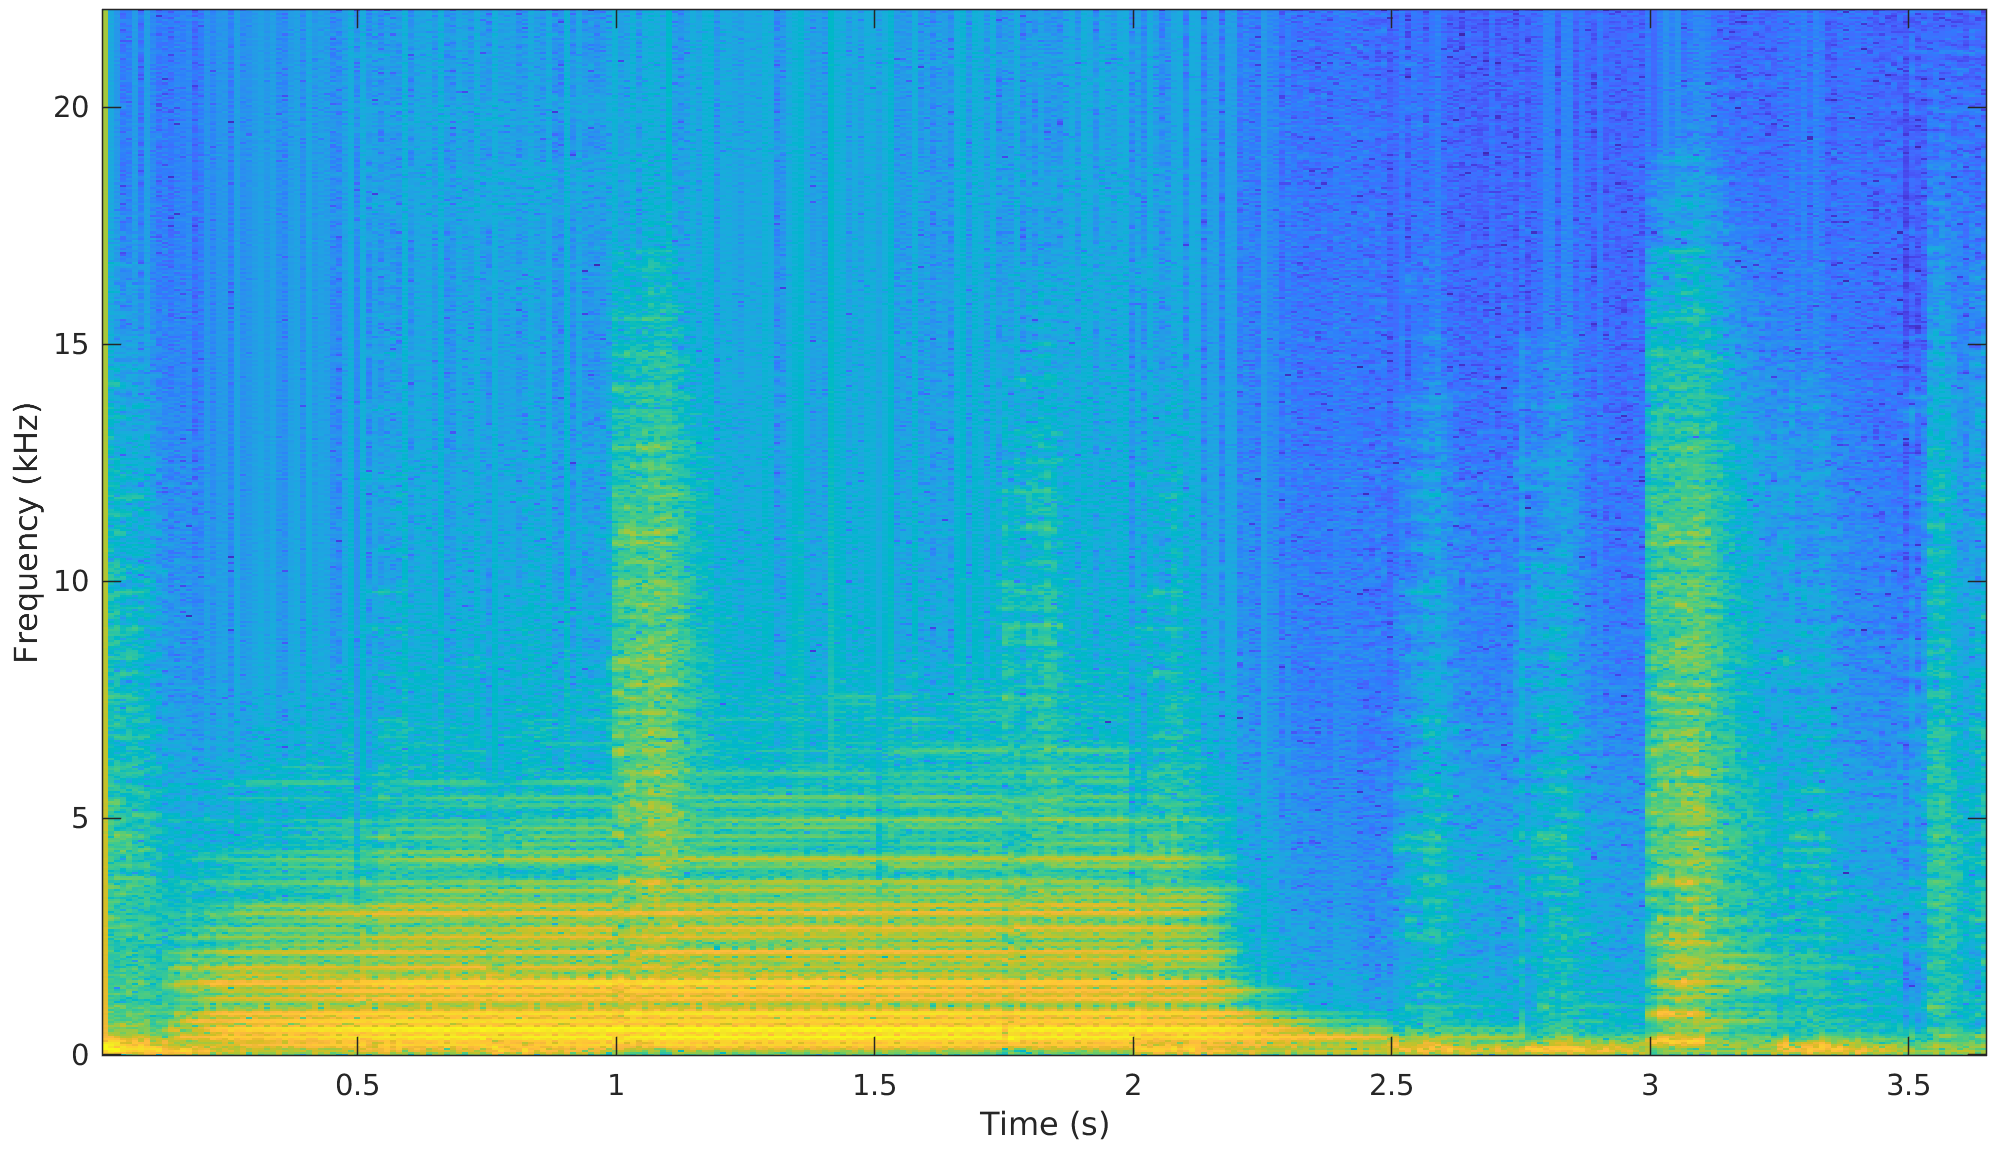
\includegraphics[width=6cm]{./harm_soft.png} }}
	\caption{Example of median-filtering HPSS}
	\label{fig:fitz1}
\end{figure}

\citet{driedger} replaced the soft mask with a binary/hard mask, and also introduced a two-pass variant. The first pass separates the harmonic component using an STFT with a large window size for high frequency resolution, followed by the second pass which separates the percussive component using an STFT with a small window size for high time resolution. \citet{fitzgerald2} created a similar iterative variant using soft masks. Additionally, they noted that when they replaced the small-window STFT with the constant-Q transform in the second pass, they obtained a separation of the human singing voice.

\subsection{TFJigsaw}

The next algorithm considered is the Time-Frequency Jigsaw Puzzle\cite{tfjigsaw}, which is implemented in the Large Time-Frequency Analysis toolbox \cite{ltfat, tfjigsaw2, tfjigsaw3}. Tonal/transient (or harmonic/percussive) separation is among one of the possible applications of TFJigsaw. The insight is similar to the iterative approach described previously -- in a TF representation with high frequency resolution, tonal sounds are well-represented, and in a TF representation with high time resolution, transient sounds are well-represented:

\begin{quote}
	[...] the starting point is to define the tonal layer of the signal as the ``component'' which admits a sparse expansion with respect to a Gabor frame with high frequency resolution (i.e. with a wide window), and the transient layer as the ``component'' which admits a sparse expansion with respect to a Gabor frame with high time resolution (i.e. a narrow window).
\end{quote}

\begin{figure}[ht]
	\centering
	\subfloat[Two lattices within a super-tile; the rectangular region is the super-tile, the ellipses represent the domains within which each TF atom's spectrogram exceeds some fixed threshold, and the dots represent their center (the TF sampling points)]{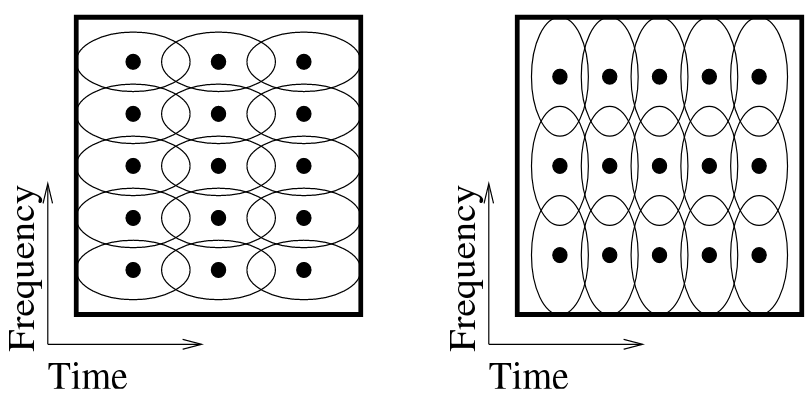
\includegraphics[height=4cm]{./tfjigsaw-supertiles.png}}
	\hspace{1em}
	\subfloat[$G^{0}$ and $G^{1}$ represent the analysis maps for the two Gabor frames, $\tilde{G}^{0}_{p}$ and $\tilde{G}^{1}_{p}$ represent the partial synthesis maps from the selected TF atoms, and $\mathcal{H}$ represents the calculation of entropy and corresponding decision]{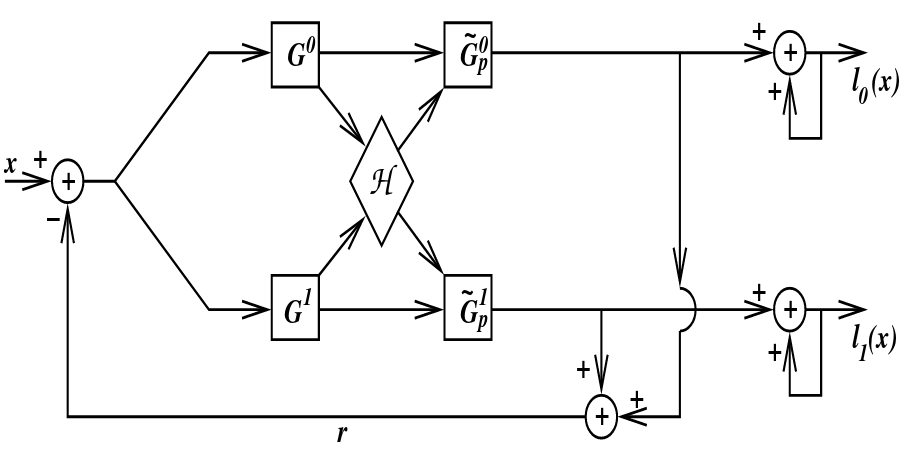
\includegraphics[height=4cm]{./tfjigsaw-entropycriterion.png}}
	\caption{\citet{tfjigsaw}'s illustrations of the TF Jigsaw Puzzle}
	\label{fig:supertiles}
\end{figure}

After creating two representations of the signal, these are superimposed in a single time-frequency plane to create so-called ``super-tiles.'' Next, within each super-tile, an entropy criterion chooses which tile (tonal or transient) is below a threshold, and subtracts these from the original signal. This is performed iteratively until the tonal and transient layers emerge. The super-tiles and entropy criterion are shown in figure \ref{fig:supertiles}, and the results are shown in figure \ref{fig:tfjigsawdemo}.

\begin{figure}[ht]
	\centering
	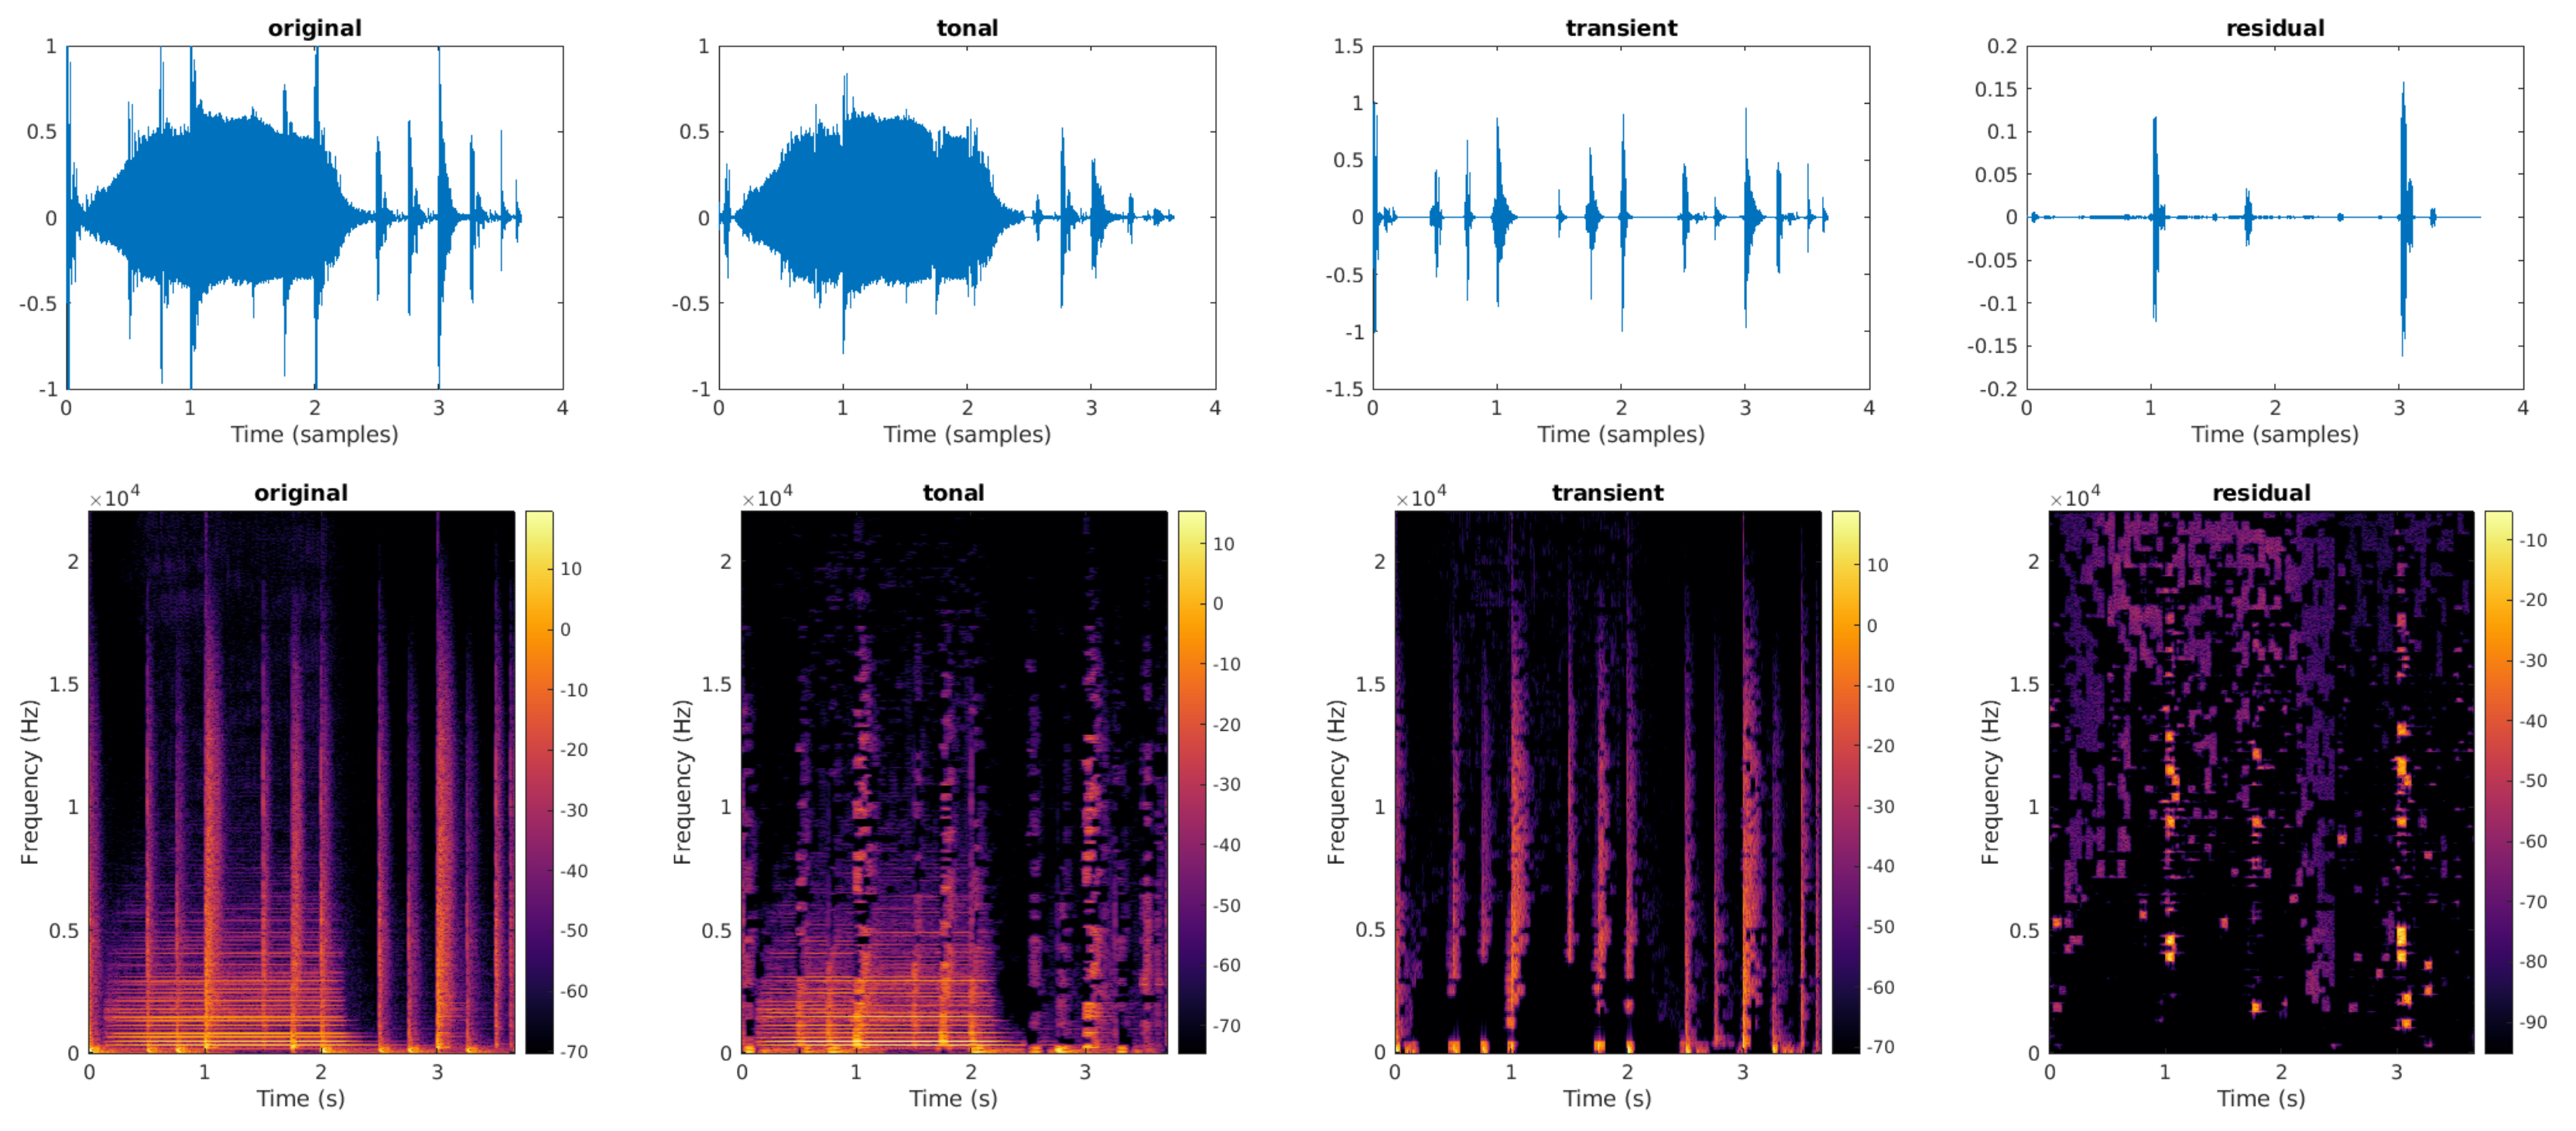
\includegraphics[width=16cm]{./tfjigsaw-sep-example.png}
	\caption{TFJigsawSep for tonal/transient separation}
	\label{fig:tfjigsawdemo}
\end{figure}

Note that the terms \textit{sparsity} and \textit{entropy} (w.r.t. TF analysis and audio signal representation) will be given a deeper treatment in section \ref{sec:theory}.

\subsection{WMDCTLasso}

The final algorithm for tonal/transient separation considered is referred to as ``WMDCTLasso.'' In LTFAT, its name is ``Audioshrink.''\cite{wmdct3}. The technique is described in a paper by \citet{wmdct}, and several demos on websites are available \cite{wmdct2, wmdct3}.

The WMDCTLasso algorithm performs a decomposition based on structured sparsity. It uses WMDCTs (Windowed Modified Discrete Cosine Transform) applied with two different time-frequency resolutions, by using a wide and narrow window -- with the wide window, the tonal sounds are well-represented, and with the narrow window, transient sounds are well-represented.

Next, a method called group lasso shrink is applied to separate the tonal and transient layers by exploiting their respective sparsity in each time-frequency representation. An example of a resulting decomposition of jazz music is shown in figure \ref{fig:wmdctex}.

\begin{figure}[ht]
	\centering
	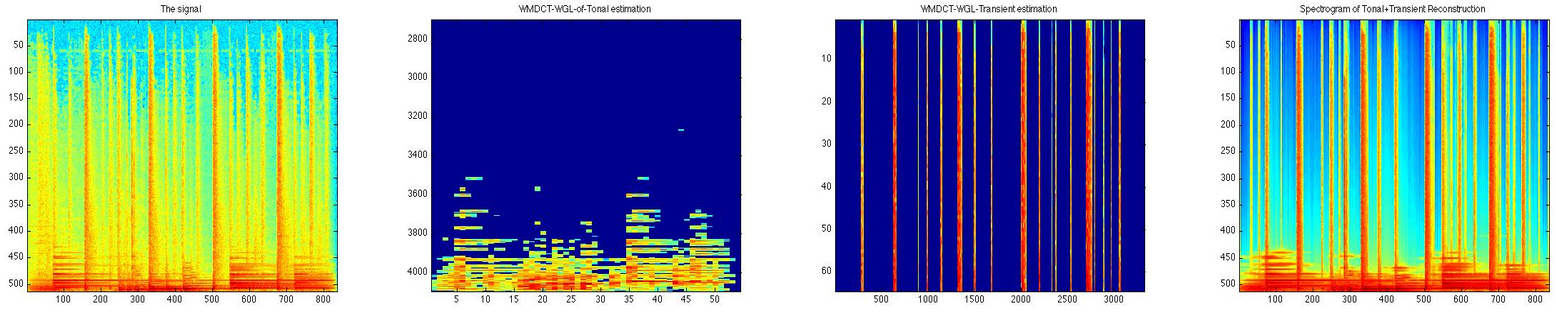
\includegraphics[width=16cm]{./wmdctjazz.png}
	\caption{WMDCTLasso for tonal/transient separation in jazz music}
	\label{fig:wmdctex}
\end{figure}

The term \textit{sparsity} is encountered again. In place of using an entropy criterion like in TFJigsaw, instead a technique called lasso shrinkage (or specifically, the group lasso variant) is used. The goal is the same -- to determine which part of the signal is best represented by the wide-window time-frequency representation, which is likely the tonal component, and similar for the case of the transient components and narrow window.

%%%%%%%%%%%%%%
% THEORY     %
%%%%%%%%%%%%%%
\section{Theory}
\label{sec:theory}

In all of the presented algorithms, there is at least one, but more commonly two, Gabor dictionaries built from the input signal, using different Gabor atoms. The STFT and CQT are well-known Gabor systems, while TFJigsaw and WMDCTLasso build their own custom Gabor dictionaries using the low-level frame functions available in LTFAT. This requires a general overview of what Gabor analysis and Gabor dictionaries are, and a demonstration of a signal represented with each of the time-frequency representations used by the different algorithms.

Second, the terms sparse signal representation and entropy are encountered in TFJigsaw and WMDCTLasso, which will be explained further. It will also be shown that the median filter used in the simpler HPSS algorithms is a form of exploiting sparsity in the time-frequency plane.

\subsection{Gabor dictionaries and time-frequency representations}

\citet{gabor1946}'s seminal signal processing paper, \textit{The Theory of Communication}, contained the first suggestion of time-frequency decomposition of a signal by applying the Fourier transform locally to overlapping portions of the signal multiplied by Gaussian windows. In other words, Gabor proposed that any signal of finite energy can be decomposed into a linear combination of time-frequency shifts of the Gaussian function. The Gabor transform $G(f)$ of a discrete-time signal $x(n)$ is described in equation (1):
\begin{flalign}
	\nonumber \mathbf{G(f)} &= [G_{1}(f), G_{2}(f), ..., G_{k}(f)]\\
	G_{m}(f) &= \sum_{n = -\infty}^{\infty}x(n)g(n-\beta m)e^{-j2\pi \alpha n},
\end{flalign}

where $g(\cdot)$ is a Gaussian low-pass window function localized at 0, $G_{m}(f)$ is the DFT of the signal centered around time $\beta m$, and $\alpha$ and $\beta$ control the time and frequency resolution of the transform. With his transform, Gabor also introduced the first formulation of the time-frequency uncertainty principle (which is minimized by using the Gaussian function as a window), stating that ``although we can carry out the analysis [of the acoustic signal] with any degree of accuracy in the time direction or frequency direction, we cannot carry it out simultaneously in both beyond a certain limit.'' Gabor called this the \textit{logon}, or smallest possible unit of time-frequency information. Mathematically, this can be stated as:
\[ \Delta t\Delta f \ge 1 \]

$\Delta t$ and $\Delta f$ are, as defined by Gabor, ``the uncertainties inherent in the definition of the epoch $t$ and frequency $f$ of an oscillation.'' The TF uncertainty principle arises from the fact that time and frequency are, in quantum physics terms, conjugate variables, or Fourier transforms of each other. This is further illustrated in figure \ref{fig:gabortf}, which shows the tiling of the time-frequency plane, and how frequency and time resolution must be sacrificed for one another by the lower bound of the time-frequency tile area.

\begin{figure}[ht]
	\centering
	\subfloat{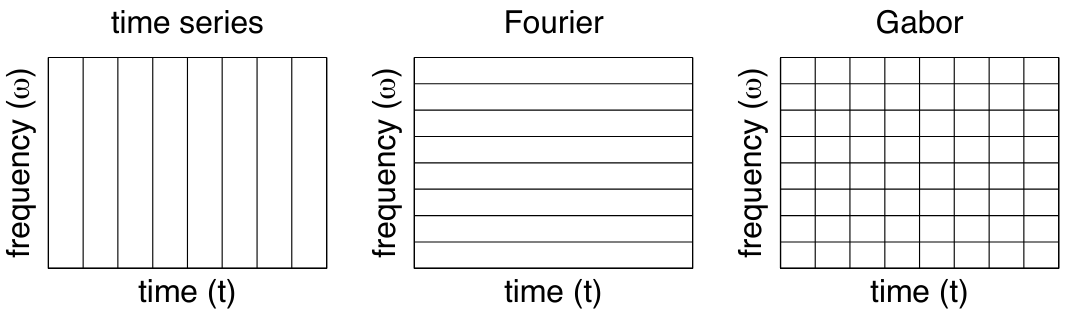
\includegraphics[height=3cm]{./gabor3.png}}
	\hspace{0.1em}
	\subfloat{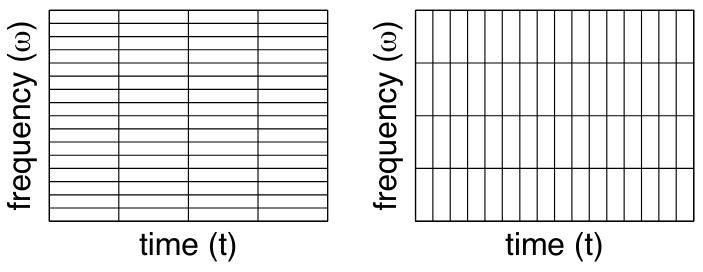
\includegraphics[height=2.56cm]{./gabor4.png}}
	\caption{A demonstration of the mutually exclusive formulations of time analysis and frequency analysis, and the lower bound of time-frequency resolution defined by Gabor's TF uncertainty principle \cite{gabordiagrams}}
	\label{fig:gabortf}
\end{figure}

Gabor noted the need for variable-frequency analysis, stating that ``the foregoing solutions [of the Fourier transform], though unquestionably mathematically correct, are somewhat difficult to reconcile with our physical intuitions and our physical concepts of such variable frequency mechanisms as, for instance, the siren.'' Similarly, psychoacoustics research shows that humans have been able to beat the time-frequency uncertainty principle \cite{psycho1, psycho2}, indicating the presence of nonlinear operators in the auditory system.

The STFT, or short-time Fourier transform, has been described independently from Gabor's work \cite{stftindie}, but additional research in the 1980s \cite{dictionary} led to the STFT being formalized and described as a special case of the Gabor transform, in recognition of Gabor's pioneering work. The STFT $X(f)$ of a discrete-time signal $x(n)$ is described in equation (2):
\begin{flalign}
	\nonumber \mathbf{X(f)} &= [X_{1}(f), X_{2}(f), ..., X_{k}(f)]\\
	X_{m}(f) &= \sum_{n = -\infty}^{\infty}x(n)g(n-mR)e^{-j2\pi f n},
\end{flalign}

where $g(\cdot)$ are the time-shifted, localized windows, $X_{m}(f)$ is the DFT of the audio signal centered about time $mR$, and $R$ is the hop size between successive time-shifts of the window. Note how similar equations (1) and (2) are, which is expected since the original Gabor transform is the STFT with a Gaussian window. Practically, the STFT allows the use of different windows and overlap sizes \cite{stftinvertible}, as long as overlap-add conditions are respected.\footnote{\url{https://www.mathworks.com/help/signal/ref/iscola.html}}

\citet{dictionary} describe the shift from the term \textit{transform}, e.g., the Gabor transform or STFT, to \textit{dictionary}, stating that works by \cite{dictionary1} and \cite{dictionary2} began the ``fundamental shift from transforms to dictionaries for sparse signal representation.'' Accordingly, an important outcome of this terminology change was the ``idea that a signal was allowed to have more than one description in the representation domain, and that selecting the best one depended on the task.'' Similar ideas were shown in \citet{doerflerphd}'s dissertation, suggesting the use of multiple Gabor dictionaries for representing music, for the two following reasons:

\begin{tight_itemize}
	\item
		\textit{Transients} are important musically, driving instrument identification and temporal events such as beats. As transients and broadband signals occur in the high frequency range, good time resolution in that range allows clearer identification of transient events.
	\item
		 Notes in the low frequency lay the harmonic basis of the song, requiring very fine frequency resolution.
\end{tight_itemize}

\citet{tfjigsaw}'s TF Jigsaw Puzzle algorithm works along these lines, establishing a multi-dictionary Gabor analysis by using two different window sizes ($R = 2$ for two dictionaries, using \citet{doerflerphd}'s terminology) for tonal and transient representation. In fact, this idea appears in most of the studied harmonic/percussive separation algorithms: the large window analysis leading to high frequency resolution for the optimal separation of pitched instruments, and the small window analysis leading to high time resolution for the optimal separation of transients.

However, \citet{doerflerphd} notes that there is a downside of high redundancy in such multi-dictionary analyses (e.g., using two STFTs is an example of high redundancy). There should be an ideal \textit{single} transform which adapts itself to the different characteristics of the signal being studied, rather than creating a new transform or dictionary for each characteristic.

The idea for a musically-appropriate single transform, the Constant-Q Transform, was first proposed by \citet{jbrown}. The goal was to create a transform which maintained a constant ratio of frequency to frequency resolution, for the following reasons:

\begin{tight_itemize}
	\item
		The harmonics of the fundamental frequency created by musical instruments have a consistent spacing in the logarithmic scale, or the \textit{constant pattern}
	\item
		Log-frequency spectra, demonstrating the constant pattern for harmonics, would be more useful in musical tasks than linear-frequency spectra
\end{tight_itemize}

This is illustrated in figure \ref{fig:violin}, showing a linear and CQT representation of violin playing a scale. Note that the musical features of the violin -- distinct notes played, even spacing between the harmonics, and the strong formant frequency in the \textasciitilde3000 Hz region -- which are clearly visible in the CQT, and not in the linear-frequency DFT.

\begin{figure}[ht]
	\centering
	\subfloat[Linear-frequency DFT]{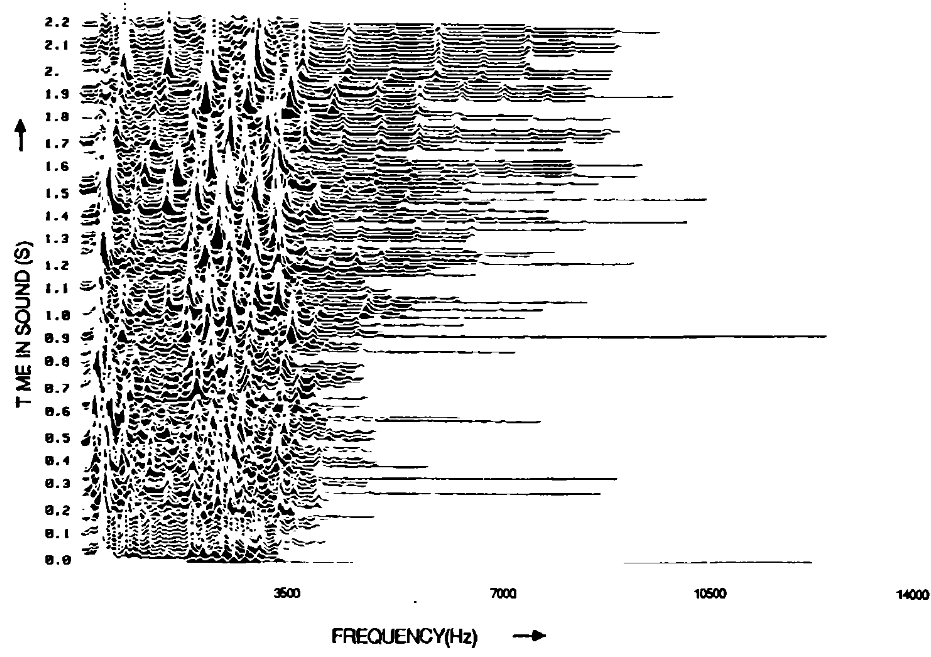
\includegraphics[height=5.2cm]{./violindft.png}}
	\hspace{0.5em}
	\subfloat[Constant-Q transform]{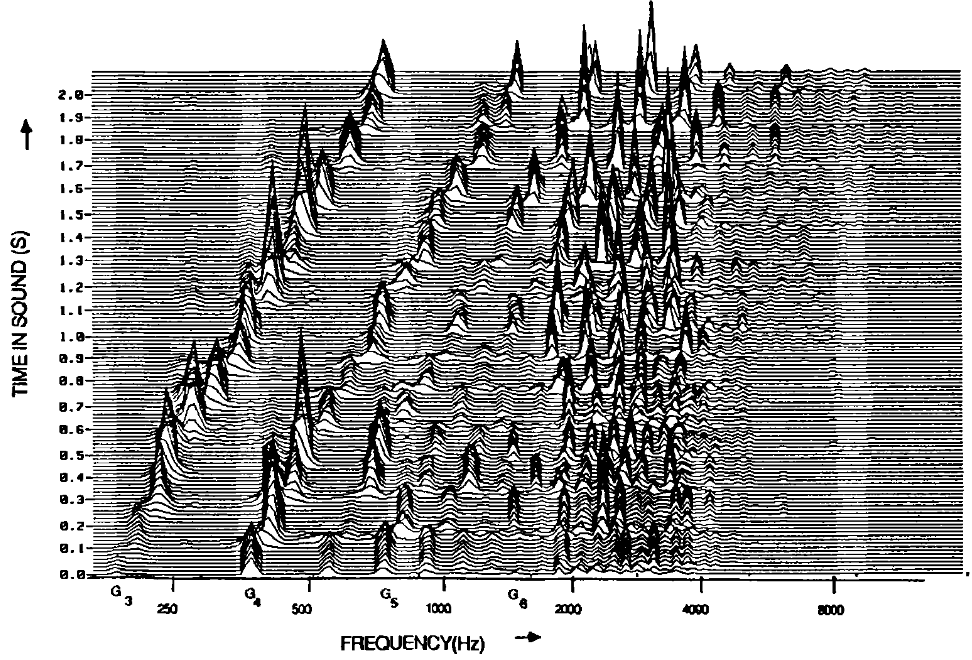
\includegraphics[height=5.5cm]{./violincqt.png}}
	\caption{Violin playing the diatonic scale, $G_{3} \text{(196Hz)} - G_{5} \text{(784Hz)}$\cite{jbrown}}
	\label{fig:violin}
\end{figure}

The first formulation of the CQT was constructed using specific window sizes for each frequency region of interest, and was not designed to be invertible, thus making it only suitable for analysis. Subsequent work by \cite{balazs, jaillet} applied formal frame theory to create a perfectly invertible and minimally redundant Constant-Q transform, by adapting the basic Gabor transform (which can also be called \textit{stationary}, since the Gaussian atoms are of a constant size with a time shift) to create the important Nonstationary Gabor Transform (NSGT, or NSDGT for the discrete-time variant).

Recall equation (1) for the discrete Gabor transform, which used time-shifted copies of identical Gaussian windows as the Gabor atoms for the decomposition:
\[ g_{m,n} = g(n-\beta m)e^{-j2\pi \alpha n} \]

The parameters $\beta$ and $\alpha$ control the time and frequency resolution of the transform. In the case of the nonstationary Gabor transform with resolution changing over time, the Gabor atoms consist of window functions selected from a set of functions $g_{m}$ using a fixed frequency sampling step $\alpha_{m}$:
\[ g_{m,n} = g_{m}(n)e^{-j2\pi \alpha_{m} n} \]

\citet{balazs} state that ``this is similar to the standard Gabor scheme [...] with the possibility to vary the window $g_{m}$ for each position $\beta_{m}$. Thus, sampling of the time-frequency plane is done on a grid which is irregular over time, but regular over frequency at each temporal position.'' Moreover, if we set $g_{m}(n) = g(n - \beta m)$ and fix the time and frequency constants $\beta$, $\alpha_{m} = \alpha$, we get back the classic form of the stationary discrete Gabor transform.

Similarly, for the nonstationary Gabor transform with resolution changing over frequency, the Gabor atoms used are selected from a set of functions $h_{n}$ using a fixed time sampling step $\beta_{n}$:
\[ h_{m,n} = h_{n}(n - \beta_{n}m) \]

\citet{balazs} state that ``in practice we will choose each function $h_{n}$ as a well-localized band-pass function with center frequency $\alpha_{m}$.'' We get back the classic form of the stationary discrete Gabor transform by selecting functions $h_{n}(n) = g(n - \beta_{n} m)e^{-j2\pi \alpha n}$ and fix the time and frequency constants $\alpha$, $\beta_{n} = \beta$.

The time-frequency lattice of the stationary and nonstationary Gabor transforms can be seen in figure \ref{fig:nsgts}.

\begin{figure}[ht]
	\centering
	\subfloat[Stationary]{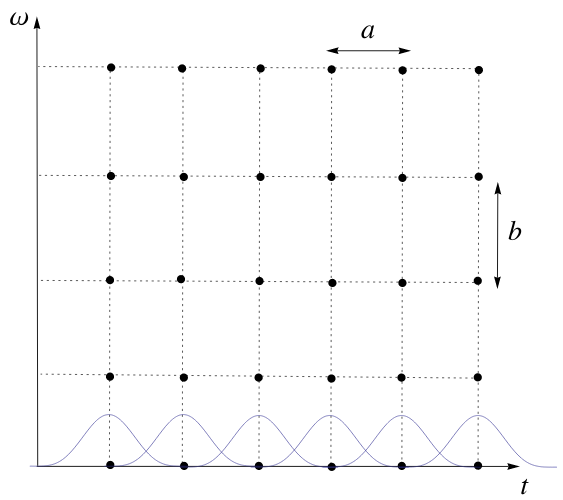
\includegraphics[height=4cm]{./sgt.png}}
	\hspace{0.35em}
	\subfloat[Nonstationary in time]{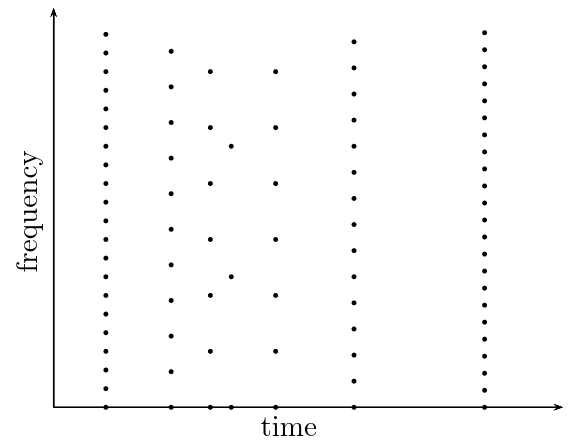
\includegraphics[height=4cm]{./nsgt_time.png}}
	\hspace{0.35em}
	\subfloat[Nonstationary in frequency]{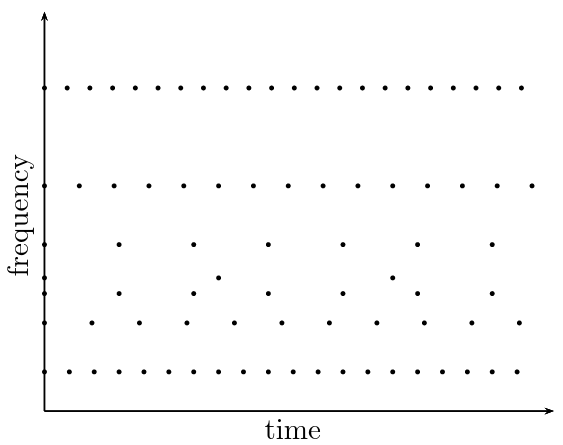
\includegraphics[height=4cm]{./nsgt_freq.png}}
	\caption{Time-frequency lattice of different Gabor transforms}
	\label{fig:nsgts}
\end{figure}

To recap, \citet{adaptivecqt} describes the concepts presented so far as follows:

\begin{quote}
	The definition of multiple Gabor frames, which is comprehensively treated in \cite{doerflerphd}, provides Gabor frames with analysis techniques with multiple resolutions. The nonstationary Gabor frames (see \cite{balazs, jaillet} for their definition and implementation) are a further development; they fully exploit theoretical properties [...], and they provide for a class of FFT-based algorithms [...] together with perfect reconstruction formulas.
\end{quote}

Several important outcomes of the NSGT were the invertible CQT with a fast FFT-based implementation \cite{invertiblecqt}, and the realtime invertible CQT \cite{rtcqt}. Aside from being available in LTFAT, the official MATLAB Wavelet Toolbox contains perfectly invertible implementations of the CQT and ICQT (inverse CQT) based on the NSGT \footnote{\url{https://www.mathworks.com/help/wavelet/ref/cqt.html}}; these transforms are used extensively throughout this paper, present in every MATLAB algorithm which uses the CQT. In the Python case, the NSGT library is used,\footnote{\url{https://github.com/grrrr/nsgt}} which contains both the invertible and realtime implementations \cite{invertiblecqt, rtcqt}.

Finally, figure \ref{fig:nsgtglock} demonstrates the advantages of the NSGT for a musical signal -- note that the small-window STFT has sharply defined time events but blurry frequency bins, and the inverse case for the large-window STFT. Finally, the NSGT contains sharp time and frequency resolution.

\begin{figure}[ht]
	\centering
	\subfloat[STFT with 6ms window]{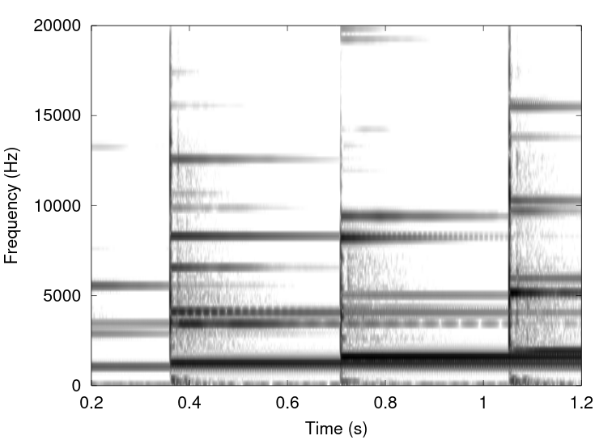
\includegraphics[height=4cm]{./tf_tradeoff_balasz1.png}}
	\hspace{0.35em}
	\subfloat[STFT with 93ms window]{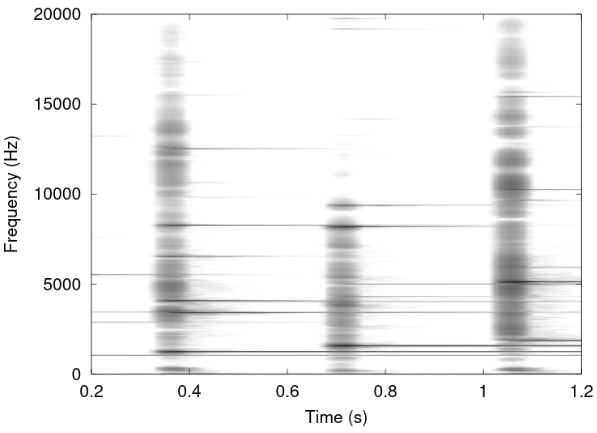
\includegraphics[height=4cm]{./tf_tradeoff_balasz2.png}}
	\hspace{0.35em}
	\subfloat[NSGT using window evolving between 6--93ms]{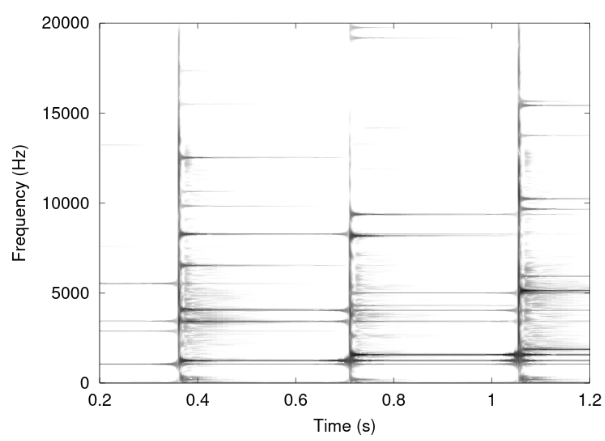
\includegraphics[height=4cm]{./tf_tradeoff_balasz3.png}}
	\caption{Transforms of a glockenspiel signal \cite{balazs}}
	\label{fig:nsgtglock}
\end{figure}

\subsection{Representations of tonal and transient sounds}

A useful exercise is to represent the classic glockenspiel signal with different dictionaries to gain some practical, hands-on experience with the characteristics, advantages, and disadvantages of each transform mentioned so far. All plots are generated with MATLAB and LTFAT.

The glockenspiel signal is well-known and useful to demonstrate transient and tonal properties of a musical signal -- it is available in the LTFAT,\footnote{\url{https://ltfat.github.io/doc/signals/gspi.html}} loaded by the \Verb#gspi# function. Figure \ref{fig:glockwaveform} shows the time-domain waveform:

\begin{figure}[ht]
	\centering
	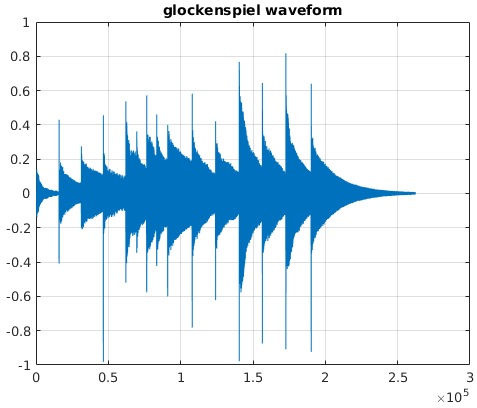
\includegraphics[height=6.5cm]{./gspi_waveform.png}
	\caption{Glockenspiel waveform}
	\label{fig:glockwaveform}
\end{figure}

Let's first consider the STFT. The standard \Verb#spectrogram# in MATLAB\footnote{\url{https://www.mathworks.com/help/signal/ref/spectrogram.html}} is computed using the short-time Fourier transform. The number of DFT output bins is set to twice the window size, and the overlap is set to half of the window size. An STFT with 3 different window sizes is shown in figure \ref{fig:glockspecs}.

\begin{figure}[ht]
	\vspace{-1em}
	\centering
	\subfloat[Window size 256]{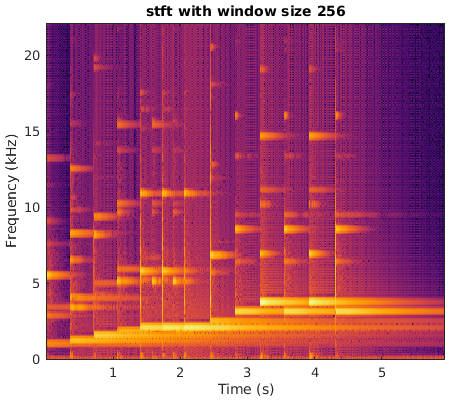
\includegraphics[height=5cm]{./glock_stft256.png}}
	\hspace{0.35em}
	\subfloat[Window size 1024]{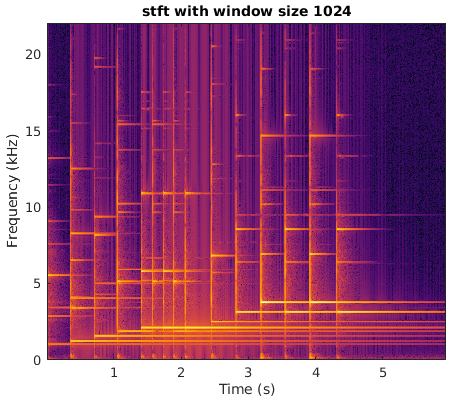
\includegraphics[height=5cm]{./glock_stft1024.png}}
	\hspace{0.35em}
	\subfloat[Window size 4096]{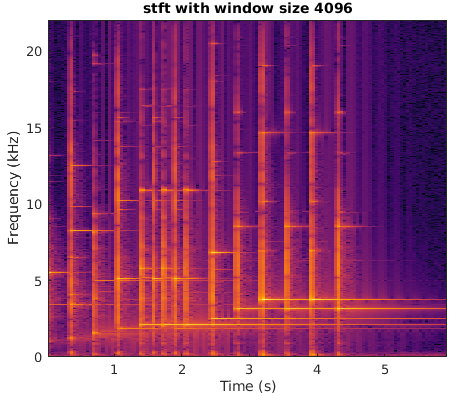
\includegraphics[height=5cm]{./glock_stft4096.png}}
	\caption{STFT-based spectrograms of the glockenspiel signal}
	\label{fig:glockspecs}
\end{figure}

The maximum frequency is the Nyquist frequency, or half the sample rate -- in this case, it is 22050 Hz (half of 44100 Hz, the gspi sample rate). The frequency resolution of the linear STFT is fixed at $\frac{\mathit{fs}}{N}$, where $\mathit{fs}$ is the sampling frequency or sample rate, and $N$ is the number of output bins of the DFT. The time resolution of the linear STFT depends on the window size. The table \ref{table:stftparams} shows the frequency resolution per window size of the STFT.

\begin{table}[ht]
	\centering
\begin{tabular}{ |l|l|l|l|c|c|c|c| }
	 \hline
	  Window size (samples) & Window size (ms) & DFT output bins & Frequency resolution (Hz) \\
	 \hline
	 \hline
	 256 & 5.8 & 512 & 86.1 \\
	 \hline
	 1024 & 23.2 & 2048 & 21.5  \\
	 \hline
	 4096 & 92.9 & 8192 & 5.4  \\
	 \hline
\end{tabular}
	\caption{STFT window sizes and frequency resolution}
	\label{table:stftparams}
\end{table}

Note that the time resolution is getting worse as the window size increases -- consider that within a window of 92.9ms, there may be several musical events occurring, such as transients or onsets, which cannot be separately distinguished, and are blurred together. However, as a tradeoff, the frequency resolution is becoming sharper -- each row of the STFT for a window of 92.9ms represents a frequency increment of 5.4Hz. Visually, we observe the time resolution of the spectrogram becoming blurrier while the frequency resolution gets sharper as the window size increases.

Next, let's consider the NSGT-CQT from the MATLAB Wavelet Toolbox function \Verb#cqt#.\footnote{\url{https://www.mathworks.com/help/wavelet/ref/cqt.html}} Various plots of the CQT are shown in figure \ref{fig:glockcqts}. Note that the bins per octave parameter controls the frequency resolution -- more bins per octave gives us a finer frequency discrimination. The Gabor atoms used to create the CQT are not constant like the STFT -- they consist of a set of window functions with different center frequencies and bandwidths to maintain the constant-Q ratio. The bins-per-octave settings shown are 12, 24, and 48, which correspond to a constant-Q ratio of $2^{\frac{1}{\text{bins}}}$, or 1.059, 1.029, and 1.014 respectively. Finally, \citet{jbrown}'s desired constant pattern in the logarithmic scale is shown in the last row of plots.

\begin{figure}[ht]
	\centering
	\subfloat[CQT spectrogram, 12 bins per octave]{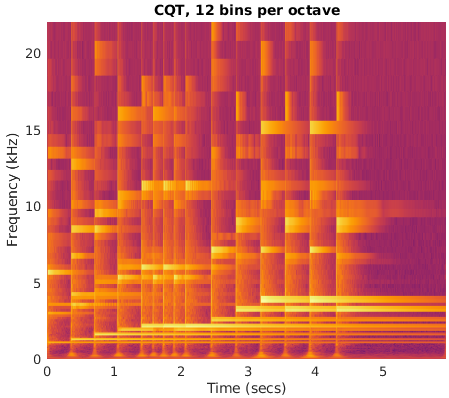
\includegraphics[height=5cm]{./glock_cqt12.png}}
	\hspace{0.35em}
	\subfloat[CQT spectrogram, 24 bins per octave]{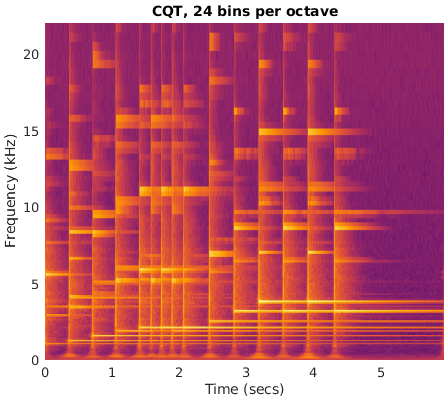
\includegraphics[height=5cm]{./glock_cqt24.png}}
	\hspace{0.35em}
	\subfloat[CQT spectrogram, 48 bins per octave]{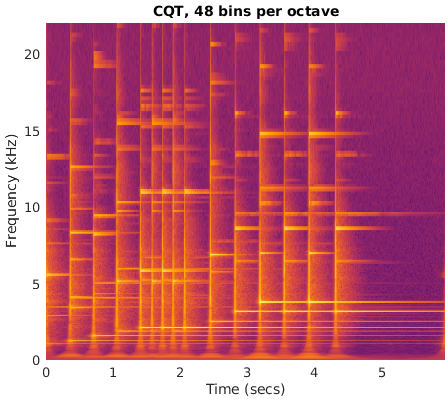
\includegraphics[height=5cm]{./glock_cqt48.png}}
	\vspace{0.1em}
	\subfloat[Ratio, 12 bins per octave]{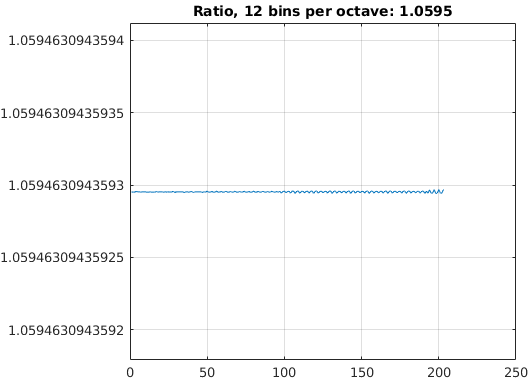
\includegraphics[height=4cm]{./glock_cqt12_ratio.png}}
	\hspace{0.35em}
	\subfloat[Ratio, 24 bins per octave]{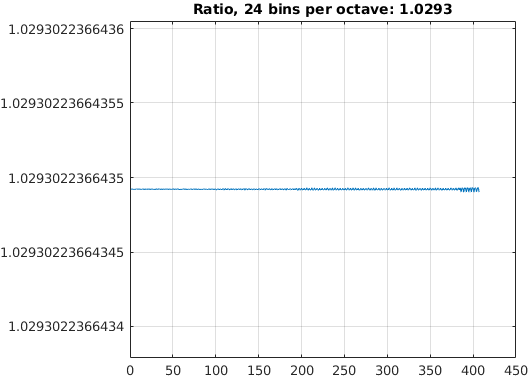
\includegraphics[height=4cm]{./glock_cqt24_ratio.png}}
	\hspace{0.35em}
	\subfloat[Ratio, 48 bins per octave]{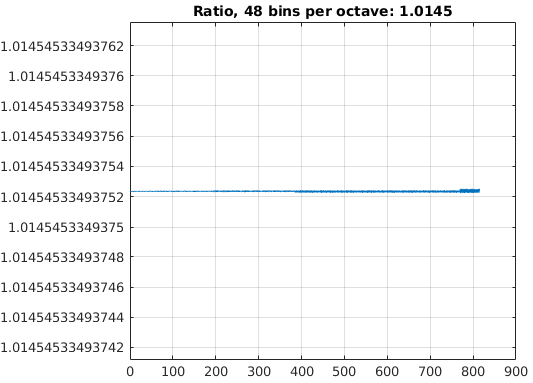
\includegraphics[height=4cm]{./glock_cqt48_ratio.png}}
	\vspace{0.1em}
	\subfloat[Gabor frame at Nyquist frequency, 12 bins per octave]{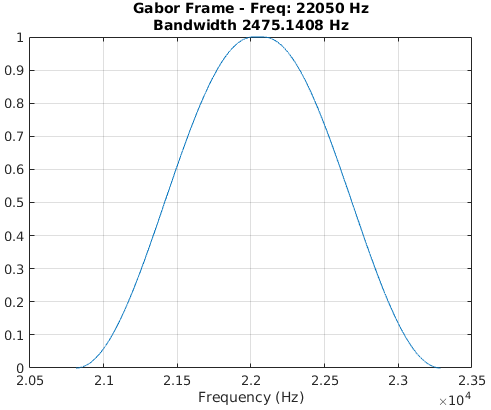
\includegraphics[height=4.5cm]{./glock_cqt12_gaborframe.png}}
	\hspace{0.35em}
	\subfloat[Gabor frame at Nyquist frequency, 24 bins per octave]{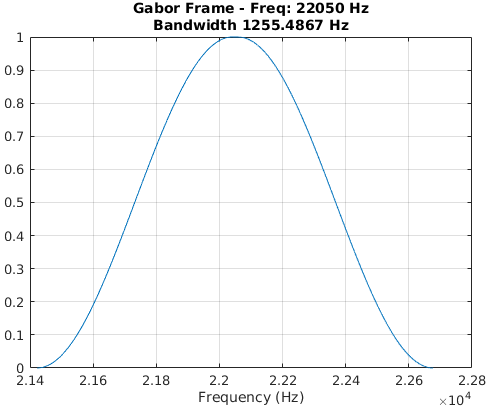
\includegraphics[height=4.5cm]{./glock_cqt24_gaborframe.png}}
	\hspace{0.35em}
	\subfloat[Gabor frame at Nyquist frequency, 48 bins per octave]{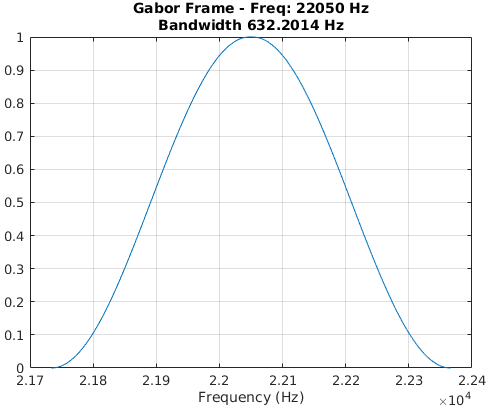
\includegraphics[height=4.5cm]{./glock_cqt48_gaborframe.png}}
	\vspace{0.1em}
	\subfloat[Center frequencies, 12 bins per octave]{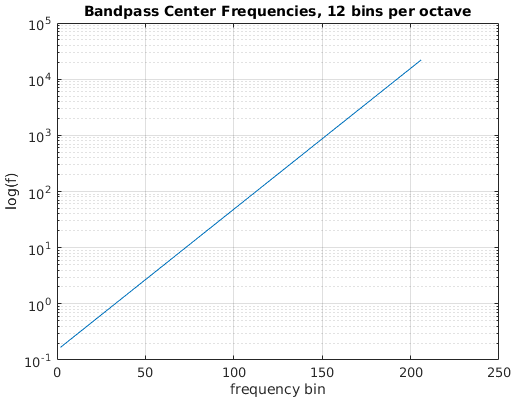
\includegraphics[height=4.25cm]{./glock_cqt12_cf.png}}
	\hspace{0.35em}
	\subfloat[Center frequencies, 24 bins per octave]{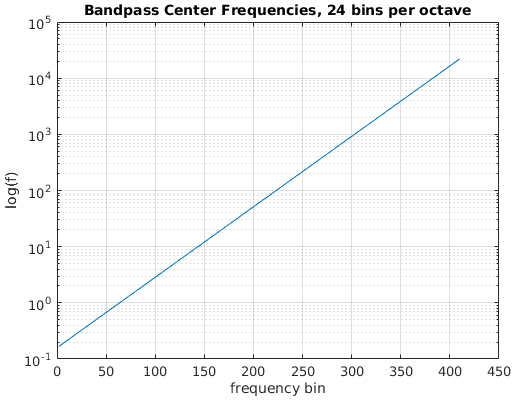
\includegraphics[height=4.25cm]{./glock_cqt24_cf.png}}
	\hspace{0.35em}
	\subfloat[Center frequencies, 48 bins per octave]{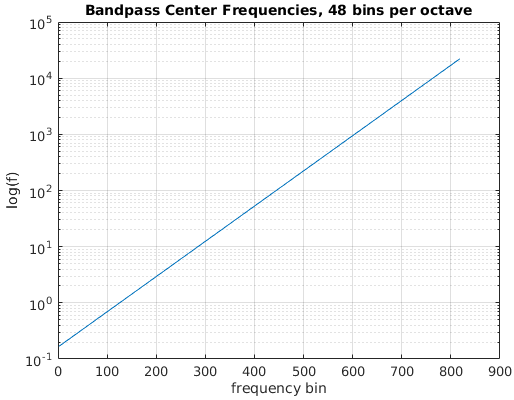
\includegraphics[height=4.25cm]{./glock_cqt48_cf.png}}
	\caption{CQT plots of glockenspiel signal}
	\label{fig:glockcqts}
\end{figure}

\clearpage
\vfill

The advantage of the CQT over the linear-frequency STFT can be seen by displaying the spectrograms side-by-side, in figure \ref{fig:cqtvstft}. Note that the CQT (regardless of bins per octave) seems to be identifying more frequency components from the glockenspiel signal, even if in the case of less bins per octave, the frequency bins are blurry. The time resolution in the CQTs is also sharp, even with high frequency resolution.

\begin{figure}[ht]
	\centering
	\subfloat[CQT spectrogram, 12 bins per octave]{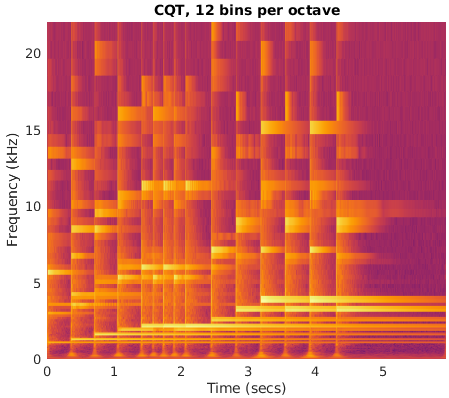
\includegraphics[height=5.25cm]{./glock_cqt12.png}}
	\hspace{0.35em}
	\subfloat[STFT spectrogram, window size 256]{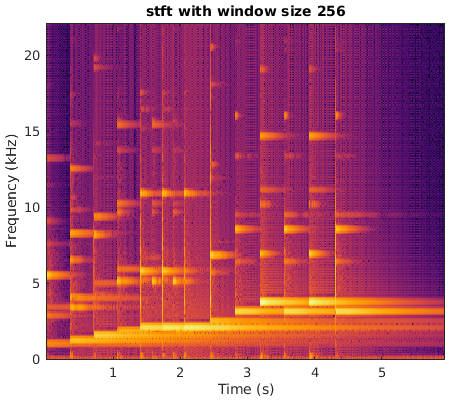
\includegraphics[height=5.25cm]{./glock_stft256.png}}\\
	\vspace{0.1em}
	\subfloat[CQT spectrogram, 24 bins per octave]{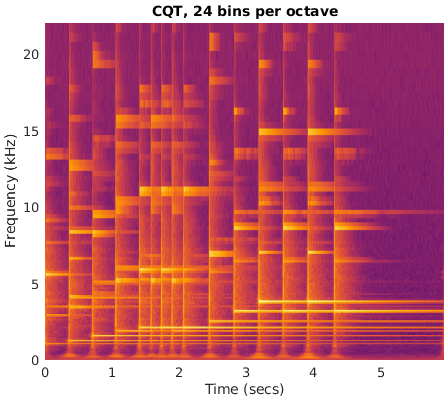
\includegraphics[height=5.25cm]{./glock_cqt24.png}}
	\hspace{0.35em}
	\subfloat[STFT spectrogram, window size 1024]{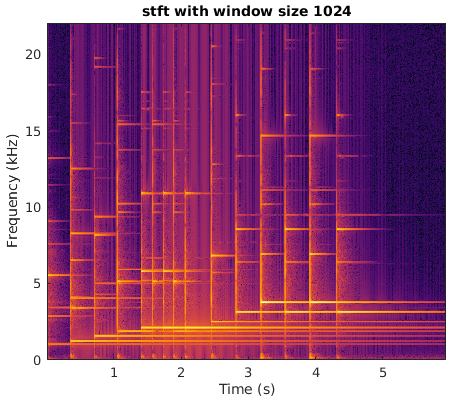
\includegraphics[height=5.25cm]{./glock_stft1024.png}}\\
	\vspace{0.1em}
	\subfloat[CQT spectrogram, 48 bins per octave]{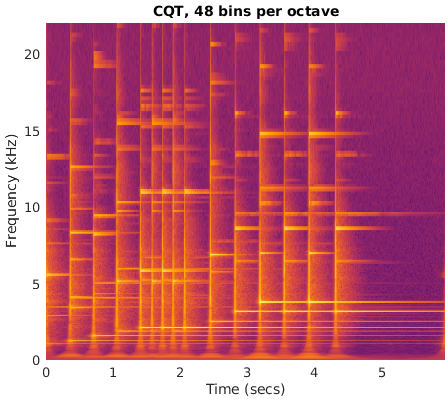
\includegraphics[height=5.25cm]{./glock_cqt48.png}}
	\hspace{0.35em}
	\subfloat[STFT spectrogram, window size 4096]{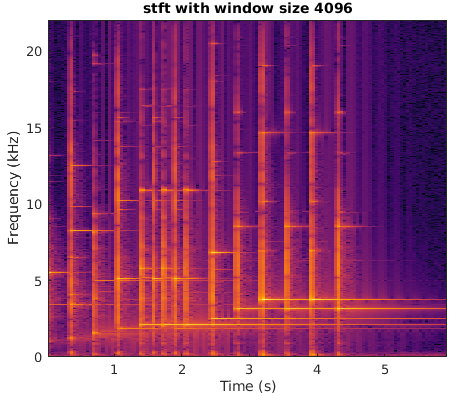
\includegraphics[height=5.25cm]{./glock_stft4096.png}}
	\caption{CQT versus STFT}
	\label{fig:cqtvstft}
\end{figure}

The final two algorithms which used custom frame-based analysis using LTFAT were the TF Jigsaw Puzzle \cite{tfjigsaw} and WMDCTLasso \cite{wmdct}. The tonal and transient systems used by TF Jigsaw are the discrete Gabor transform with a Hann window of size 4096 samples and 256 samples respectively. The tonal and transient systems used by WMDCTLasso are the WMDCT transform with a Gaussian window of 256 and 32 channels respectively. These are implemented in LTFAT\footnote{\url{https://ltfat.github.io/doc/gabor/wmdct.html}, \url{https://ltfat.github.io/doc/gabor/dgtreal.html}} and shown in figure \ref{fig:frametransforms}.

\begin{figure}[ht]
	\centering
	\subfloat[Tonal DGTReal]{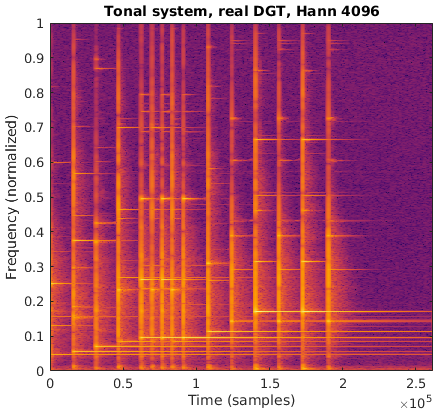
\includegraphics[height=5.25cm]{./glock_dgtreal_tonal.png}}
	\hspace{0.35em}
	\subfloat[Transient DGTReal]{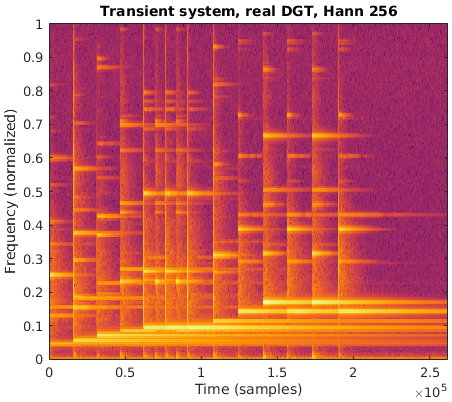
\includegraphics[height=5.25cm]{./glock_dgtreal_transient.png}}
	\vspace{0.1em}
	\subfloat[Tonal WMDCT]{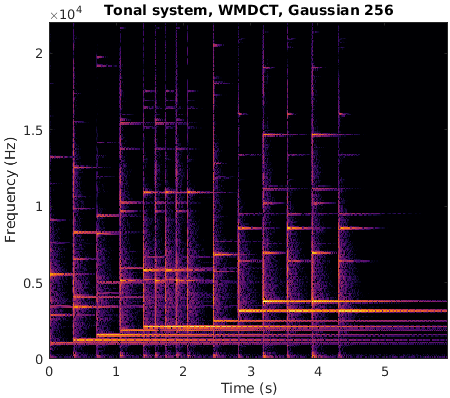
\includegraphics[height=5.25cm]{./glock_wmdct_tonal.png}}
	\hspace{0.35em}
	\subfloat[Transient WMDCT]{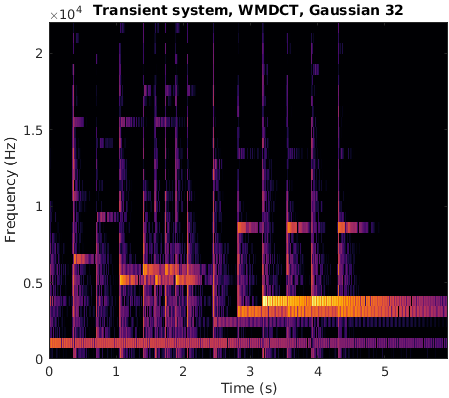
\includegraphics[height=5.25cm]{./glock_wmdct_transient.png}}
	\caption{Tonal and transient systems used by TF Jigsaw and WMDCTLasso for the glockenspiel signal}
	\label{fig:frametransforms}
\end{figure}

The DGTReal is simply the STFT or short-time Fourier transform. The WMDCT is a transform that minimizes redundancy -- the DFT decomposes a signal into complex exponentials, and the DCT decomposes a signal into real cosines. For a more rigorous treatment on the MDCT in relation to the DFT, refer to \cite{mdct}. In short, a \textit{critically sampled} transform is one where the number of transformed samples is equal to the number of time-domain input samples -- considering the STFT, this would be achieved with non-overlapping rectangular windows. However, this suffers poor frequency resolution and block effects after inverting modifications to the transform. Overlapping transforms (such as an STFT with a Hann window and overlap of 50\% window size) contain redundancy. The WMDCT is critically sampled and avoids block effects with time-domain aliasing cancellation. The difference can be observed visually by noticing there is more empty (or black) area in the WMDCT spectrogram, indicating lower redundancy.

\clearpage
\vfill

\subsection{Time-frequency masking}

Surveys on speech \cite{speechmask} and music separation \cite{musicmask} indicate that the majority of separation algorithms use the technique of time-frequency masking (or spectral masking) to separate the sources. The median-filtering algorithms of \citet{fitzgerald1, fitzgerald2, driedger} all use time-frequency masking.

\begin{wrapfigure}{r}{8cm}
	\vspace{-1.0em}
	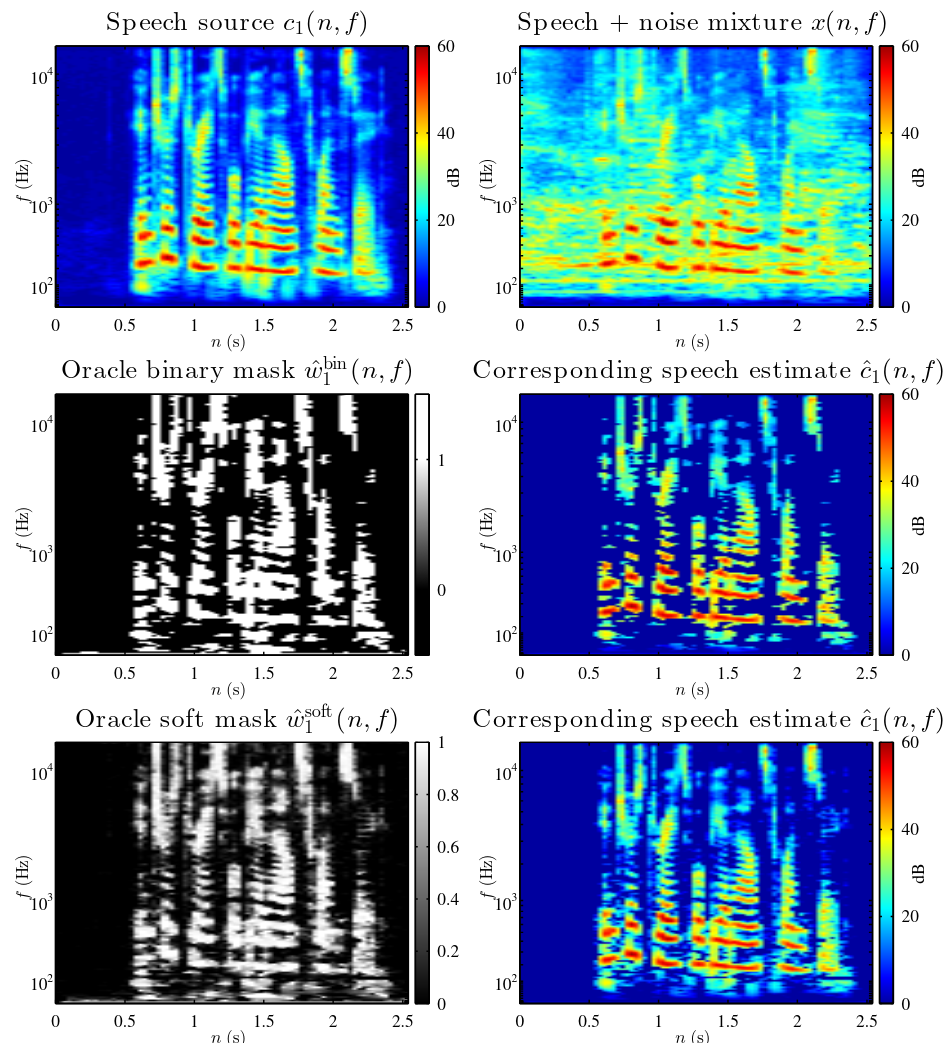
\includegraphics[width=8cm]{./maskdemo.png}
	\caption{Results of a soft and hard oracle mask applied for speech denoising. The oracle mask is the ideal mask for a given signal -- to compute it, the target and interference signals must be known.}
	\label{fig:masks}
	\vspace{-1.5em}
\end{wrapfigure}

\citet{masking} describe different time-frequency masking strategies in audio source separation. A time-frequency mask (or spectral mask, or masking filter) is a matrix of the same size as the complex STFT, by which the STFT is multiplied to mask, filter, or suppress specific time-frequency bins. A soft mask has real values $\in [0, 1]$, and a binary or hard mask has logical values, i.e., only 0 and 1. The soft mask used in \cite{fitzgerald1, fitzgerald2} is a Wiener filter given in the following equation, where $\hat{S}$ represents the complex-valued spectrogram:
\[ M = \frac{|\hat{S}_{\text{target}}|^{2}}{|\hat{S}_{\text{interference}}|^{2} + |\hat{S}_{\text{target}}|^{2}} \]

The hard mask used in \cite{driedger} is of the form:
\[ M = \frac{|\hat{S}_{\text{target}}|}{|\hat{S}_{\text{interference}}| + \epsilon} \le \beta \]

, where $\beta$ is the separation factor. Note the inclusion of machine epsilon in the denominator, to avoid division by zero. One advantage of the hard mask's separation factor is that a third component can be extracted. Let's reformulate the hard mask formula in the harmonic/percussive case to present a concrete example:
\[ M_{\text{harmonic}} = \frac{|\hat{S}_{\text{percussive}}|}{|\hat{S}_{\text{harmonic}}| + \epsilon} > \beta \]
\[ M_{\text{percussive}} = \frac{|\hat{S}_{\text{harmonic}}|}{|\hat{S}_{\text{percussive}}| + \epsilon} \ge \beta \]

In the median-filtering algorithms, the harmonic and percussive spectrogram estimates are the output of the median filtering step. By setting $\beta > 1$, we are stating that the harmonic and percussive estimates must be at least $\beta$ different from each other -- this gives us the capability to extract a third component, called the residual:
\[ M_{\text{residual}} = 1 - (M_{\text{harmonic}} + M_{\text{percussive}}) \]

Soft masks generally produce higher quality sound. An illustration of spectral masking is shown in figure \ref{fig:masks}.

\subsection{\textbf{\textcolor{red}{TODO }}Sparsity, entropy, and matching pursuit}
\label{sec:theorysparsity}

\textbf{\textcolor{red}{TODO }}Median filtering as matching pursuit

\vfill
\clearpage

%%%%%%%%%%%%%%%
% METHODOLOGY %
%%%%%%%%%%%%%%%
\section{Methodology}
\label{sec:methodology}

\subsection{Objective measures}

The SigSep\footnote{\url{https://sigsep.github.io/}} community, borrowing from the methodology of Signal Separation Evaluation Campaign (SISEC), uses the BSS (Blind Source Separation) Eval \cite{bss} objective measure for separation quality. The authors of BSS released an improved version that matches better with subjective human evaluations, which they called the PEASS (Perceptual Evaluation methods for Audio Source Separation) Toolkit \cite{peass}, based on PEMO-Q \cite{pemoq}. The PEASS Toolkit for MATLAB \cite{peassmatlab} conveniently includes all 3 measures: PEASS, PEMO-Q, and BSS. Each of these consist of 4 metrics:

\begin{tight_itemize}
\item
	\textbf{Target:} measure of desired sound in the separation. TPS (Target Perceptual Score) in PEASS, ISR (source Image to Spatial distortion Ratio) in BSS, qTarget in PEMO-Q.
\item
	\textbf{Interference:} measure of undesired sounds in the separation. IPS (Interference Perceptual Score) in PEASS, SIR (Signal to Interference Ratio) in BSS, qInterf in PEMO-Q.
\item
	\textbf{Artifacts:} measure of artifacts in the separation. APS (Artifact Perceptual Score) in PEASS, SAR (Signal to Artifacts Ratio) in SAR, qArtif in PEMO-Q.
\item
	\textbf{Global:} a global score for the previous three. In PEASS, this is OPS (Overall Perceptual Score). In BSS, this is SDR (Signal to Distortion Ratio). In PEMO-Q, this is qGlobal.
\end{tight_itemize}

\citet{beassvpeass} make the recommendation to use PEASS for music separation evaluation, noting the importance of perception in music applications. They also recommend to evaluate algorithms based on their separate target, interference, and artifact scores, noting that the global measure of OPS (for PEASS) and SDR (for BSS) have an uncertain relation to the three constituent scores. The choice in this paper is to use the three individual metrics from the PEASS:
\begin{tight_enumerate}
	\item
		\textbf{TPS} (Target Perceptual Score)
	\item
		\textbf{APS} (Artifact Perceptual Score)
	\item
		\textbf{IPS} (Interference Perceptual Score)
\end{tight_enumerate}

\subsection{Evaluated music}

The most popular music stem dataset used by SISEC and SigSep is the MUSDB18 dataset \cite{musdb18} (or the HQ, high-quality, equivalent \cite{musdb18-hq}). MUSDB18-HQ contains stereo wav files sampled at 44100 Hz representing stems (drum, vocal, bass, and other) from a collection of permissively licensed music, specifically intended for recording, mastering, mixing (and in this case, ``de-mixing'', or source separation) research. 

A limited subset of MUSDB18-HQ was evaluated, or 5 total minutes of music, consisting of 4 segments of 15 seconds duration taken from 5 separate tracks. The algorithms are sample rate agnostic, so the sample rate of MUSDB18-HQ is used (44100 Hz). For simplicity, only mono audio is supported in the algorithms, and the conversion from stereo to mono is done in the Python wav segmentation script. One data set was prepared for harmonic/percussive separation evaluation (vocals omitted from the mix), and one data set for harmonic/percussive/vocal evaluation (vocals are present). The evaluation was limited to 5 minutes of music since the PEASS measure is computationally expensive.

The songs in the MUSDB18-HQ dataset are split into train and test sets. Since the final comparison of this paper will consider a neural network model which was trained on MUSDB18, the evaluation data is taken from the test set -- if we took it from the training set, the neural network could overfit and overperform.

\subsection{Evaluation format}

Due to the large number of algorithms and configurations that will be evaluated, introducing them all at the same time will be overwhelming, and will make it difficult to form conclusions. The proposed format will be like an ``elimination tournament,'' similar to sports tournaments. Starting from the simplest one-pass algorithm for harmonic/percussive source separation, we can perform evaluations to form intermediate conclusions:

\begin{tight_itemize}
\item
	Is the STFT or CQT better for harmonic/percussive source separation
\item
	Which window size of STFT (out of 128, 256, 1024, 2048, 4096, 16384), or which bins-per-octave of CQT (12, 24, 48, 96), performs best
\item
	Which of soft or hard masking performs best
\end{tight_itemize} 

From these, we can move on to two-pass variants, by using the conclusions from the previous evaluation. Next, we can evaluate the TF jigsaw and WMDCT group lasso methods with different configurations. After the harmonic/percussive evaluations are done, we can introduce vocal separation, and repeat. The initial evaluations will be described in the following section, \ref{sec:elim}.

The final goal is to combine the best performers to create optimal ``hybrid'' algorithms for each task: HPSS and harmonic/percussive/vocal separation. At the last stage, the optimal hybrids will be compared to Open-Unmix \cite{umx}. Open-Unmix is a deep-learning-based music source separation system which achieves near state-of-the-art results. It is fully open-source, and was intended to be a reference and benchmark in the field of signal separation.

\subsection{Python/MATLAB testbench}

The language chosen to implement the algorithms was MATLAB. It is an obvious choice since it has access to LTFAT, the PEASS Toolkit, many other signal processing tools (e.g., Wavelet Toolbox), and is in general a natural choice for prototyping digital signal processing algorithms. On the other hand, certain tasks for the project are more easily accomplished with Python. One example is in the preparation of the datasets, which requires traversing directories of stem files to produce mix and reference harmonic/percussive/vocal files. Also, Python would be a good choice for data visualization and result aggregation, to be able to use numpy\cite{numpy}, pandas\cite{pandas}, matplotlib\cite{matplotlib}, and seaborn\cite{seaborn}. The solution is to employ both languages wherever appropriate, and use the file system and JSON as universal interchanges:
\begin{tight_enumerate}
\item
	The Python script for data preparation scans the stem directories of MUSDB18-HQ, creates test wav files for each of the mixed and individual source signals, with a prefix indicating a unique sequence number.
\item
	The MATLAB testbench script finds all mix files, executes the separation algorithms being tested on each, and writes the separated component outputs to a directory with the algorithm name, e.g., ``1pass-hpss-f-cqt-24,'' for easy identification.
\item
	The MATLAB testbench script calculates the median PEASS scores across all of the testcases, and prints a JSON-encoded string containing the algorithm names and scores.
\item
	The Python result analysis script takes the JSON string as an input, and produces heatmaps for reporting and visualization.
\end{tight_enumerate}

One final issue is that Open-Unmix, the deep learning solution chosen as a reference, is implemented for Python with pytorch\cite{pytorch}. The solution was to write a MATLAB shim script for Open-Unmix, which uses the `system' command in MATLAB to run Open-Unmix using the operating system's Python interpreter. In this way, every algorithm could be executed by the MATLAB testbench.

%%%%%%%%%%%%%%%%%%%%%%%%%%
% Evaluations %
%%%%%%%%%%%%%%%%%%%%%%%%%%
\section{Algorithm evaluations}
\label{sec:elim}

\textbf{N.B.:} as a shorthand, STFT with window size X will be referred to as STFT-X, and CQT with bins-per-octave X will be referred to as CQT-X. For example, CQT-96 is a CQT with 96 bins-per-octave, and STFT-2048 is an STFT with window size 2048.

\subsection{Harmonic/percussive source separation}

The first task is harmonic/percussive source separation. The mixtures are combined from the instrument stems (excluding vocals). The evaluation is performed on 5 minutes of music from MUSDB18-HQ, as was mentioned. The results are displayed as colored heatmaps, where green is the best result and red is the worst. This enables a quick visual verification of the best performers.

\subsubsection{Median-filtering with STFT/CQT masking}
\label{subsec:mfilthpss}

We can consider two generalized frameworks for harmonic/percussive (and optionally vocal) source separation with masking and median filtering of either the STFT and CQT, considering the one-pass and two-pass variants separately. In both cases, we can substitute different window sizes of STFT, or the CQT with different bins per octave, to test the effects. The block diagram of the system under test is shown in figure \ref{fig:fitz2}, and the algorithms are described in listing \ref{lst:pseudocodes}.

\begin{figure}[ht]
	\centering
	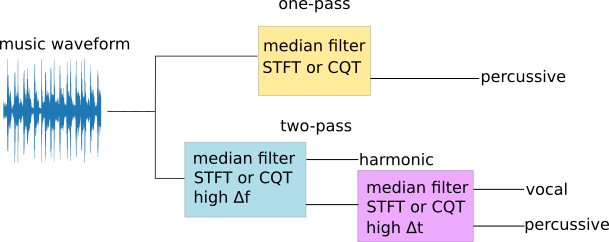
\includegraphics[width=10cm]{./medianfiltdiagram.png}
	\caption{A general framework for median filtering music separation}
	\label{fig:fitz2}
\end{figure}

The first and original median-filtering HPSS algorithm with soft masks was introduced by \citet{fitzgerald1}. The modification introduced by \citet{driedger} uses hard masks (the same paper contains the two-pass variant, which will be discussed later).

\begin{figure}[h]
  \centering
 \begin{minipage}{0.48\textwidth}
  \centering
\begin{minted}[numbersep=\mintednumbersep,linenos,mathescape=true,breaklines,frame=single,escapeinside=||]{text}
|$s = \text{mixed audio}$|
|$\hat{S} = \text{STFT}(s)\text{\textbf{ or CQT}}$|
|$S = \text{abs}(\hat{S})$|
|$H = \text{medianfilter}(S, l_{H}, \text{axis}=2)$|
|$P = \text{medianfilter}(S, l_{P}, \text{axis}=1)$|
|$\text{\textbf{soft} } M_{H} = \frac{H^{p}}{H^{p} + P^{p}}, M_{P} = \frac{P^{p}}{H^{p} + P^{p}}$|
|$\text{\textbf{hard} } M_{H} = \frac{H}{P + \epsilon} \ge \beta, M_{P} = \frac{P}{H + \epsilon} > \beta$|
|$\hat{H} = \hat{S} \cdot M_{H}$|
|$\hat{P} = \hat{S} \cdot M_{P}$|
|$h = \text{ISTFT}(\hat{H})\text{\textbf{ or ICQT}}$|
|$p = \text{ISTFT}(\hat{P})\text{\textbf{  or ICQT}}$|
\end{minted}
 \end{minipage}
\hspace{0.02\textwidth}
 \begin{minipage}{0.48\textwidth}
  \centering
\begin{minted}[numbersep=\mintednumbersep,linenos,mathescape=true,breaklines,frame=single,escapeinside=||]{text}
|$s = \text{mixed audio}$|
|$\hat{S1} = \text{STFT}(s, \text{window}=4096)\text{\textbf{ or CQT}}$|
|$ \text{apply one-pass algorithm to get } \hat{H1}, \hat{P1} $|
|$\text{\textbf{final harmonic} } h1 = \text{ISTFT}(\hat{H1})\text{\textbf{ or ICQT}}$|
|$p1 = \text{ISTFT}(\hat{P1})\text{\textbf{ or ICQT}}$|
|$\hat{S2} = \text{STFT}(p1, \text{window}=256)\text{\textbf{ or CQT}}$|
|$ \text{apply one-pass algorithm to get } \hat{H2}, \hat{P2} $|
|$h2 = \text{ISTFT}(\hat{H2})\text{\textbf{ or ICQT}}$|
|$\text{\textbf{final percussive} } p1 = \text{ISTFT}(\hat{P2})\text{\textbf{ or ICQT}}$|
\end{minted}
 \end{minipage}
  \captionof{listing}{1- and 2-pass median-filtering HPSS algorithms}
  \label{lst:pseudocodes}
\end{figure}

Some parameters are fixed in the evaluation, since they're not relevant to time-frequency resolution. Median filter lengths of $l_{H} = l_{P} = 17$ were used for the STFT, and $l_{H} = 17, l_{P} = 7$ for the CQT (as suggested in \cite{fitzgerald1, fitzgerald2}). The power for the soft masking was set to $p = 2$, and the separation factor for the hard masking was set to $\beta = 2$ (as suggested in \cite{fitzgerald1, driedger}). The results can be seen in figures \ref{fig:round1soft} and \ref{fig:round1hard}. The naming scheme for the tested configurations is described in table \ref{table:round1hpss}.

\begin{table}[ht]
	\centering
\begin{tabular}{ |l|l|c|c| }
	 \hline
	  Name & Configuration \\
	 \hline
	 \hline
	 x1pass\_hpss\_f\_\{128-16384\} & 1-pass Fitzgerald (soft mask) with STFT of size 128-16384 \\
	 \hline
	 x1pass\_hpss\_f\_cqt\_\{12-96\} & 1-pass Fitzgerald (soft mask) with CQT of bins-per-octave 12-96 \\
	 \hline
	 x1pass\_hpss\_d\_\{128-16384\} & 1-pass Driedger (hard mask) with STFT of size 128-16384 \\
	 \hline
	 x1pass\_hpss\_d\_cqt\_\{12-96\} & 1-pass Driedger (hard mask) with CQT of bins-per-octave 12-96 \\
	 \hline
\end{tabular}
	\caption{One-pass HPSS configuration naming scheme}
	\label{table:round1hpss}
\end{table}

With soft masking, using CQT-96 achieves the best score in both the harmonic and percussive separation's target, and is the best performer from all variants in percussive separation. In the harmonic separation, the evaluated STFT configurations showed better interference and worse artifacts compared to the CQT configurations. With hard masking, all of the evaluations showed poor target and artifact scores. This is consistent with the quality of soft versus hard time-frequency masking mentioned in the masking overview \cite{masking} in the introduction. CQT-96 outperforms all the STFTs for harmonic separation in the hard masking algorithm. The STFT-2048 performs the best at percussive separation.

CQT-96 demonstrates good results for both harmonic and percussive separation with soft masks, indicating it has both desired qualities: high frequency resolution, originally achieved with a large-window STFT, and high time resolution, originally achieved with a small-window STFT. This makes it a good choice for one-pass harmonic/percussive source separation.

\begin{figure}[ht]
	\centering
	\makebox[\textwidth]{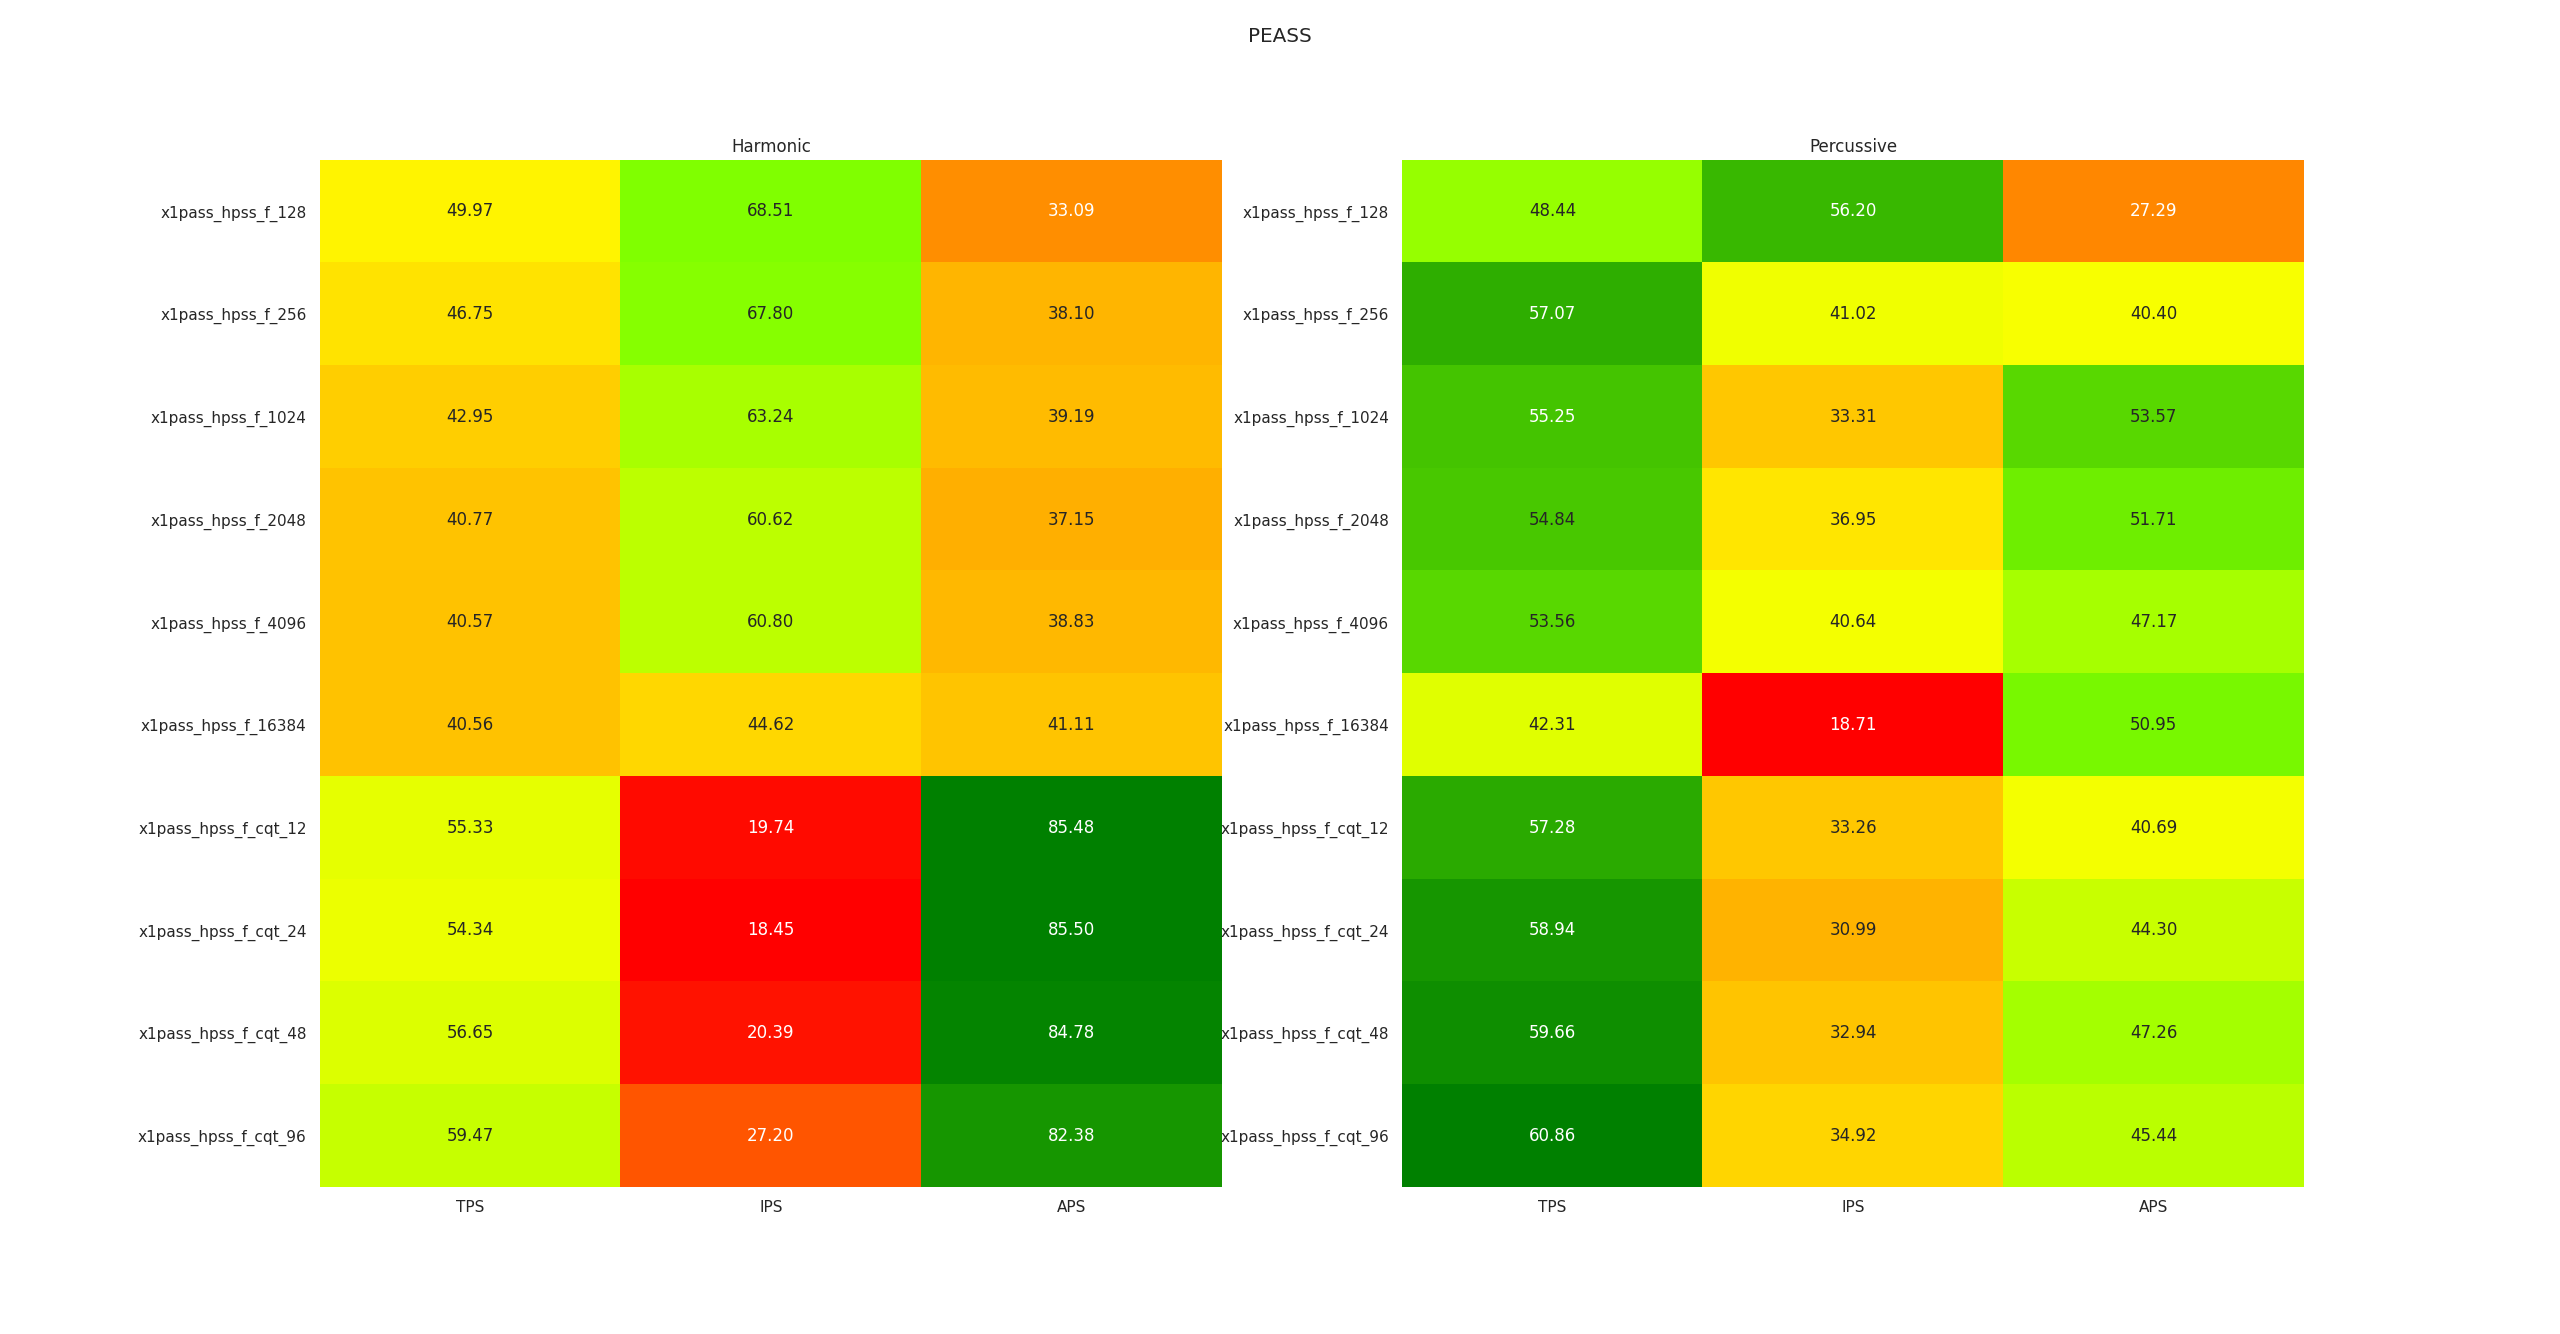
\includegraphics[width=16cm]{../evaluation/heatmaps/1pass_Fitzgerald_PEASS_abbrev.png}}
	\caption{One-pass soft-masking PEASS results}
	\label{fig:round1soft}
\end{figure}

\begin{figure}[ht]
	\centering
	\makebox[\textwidth]{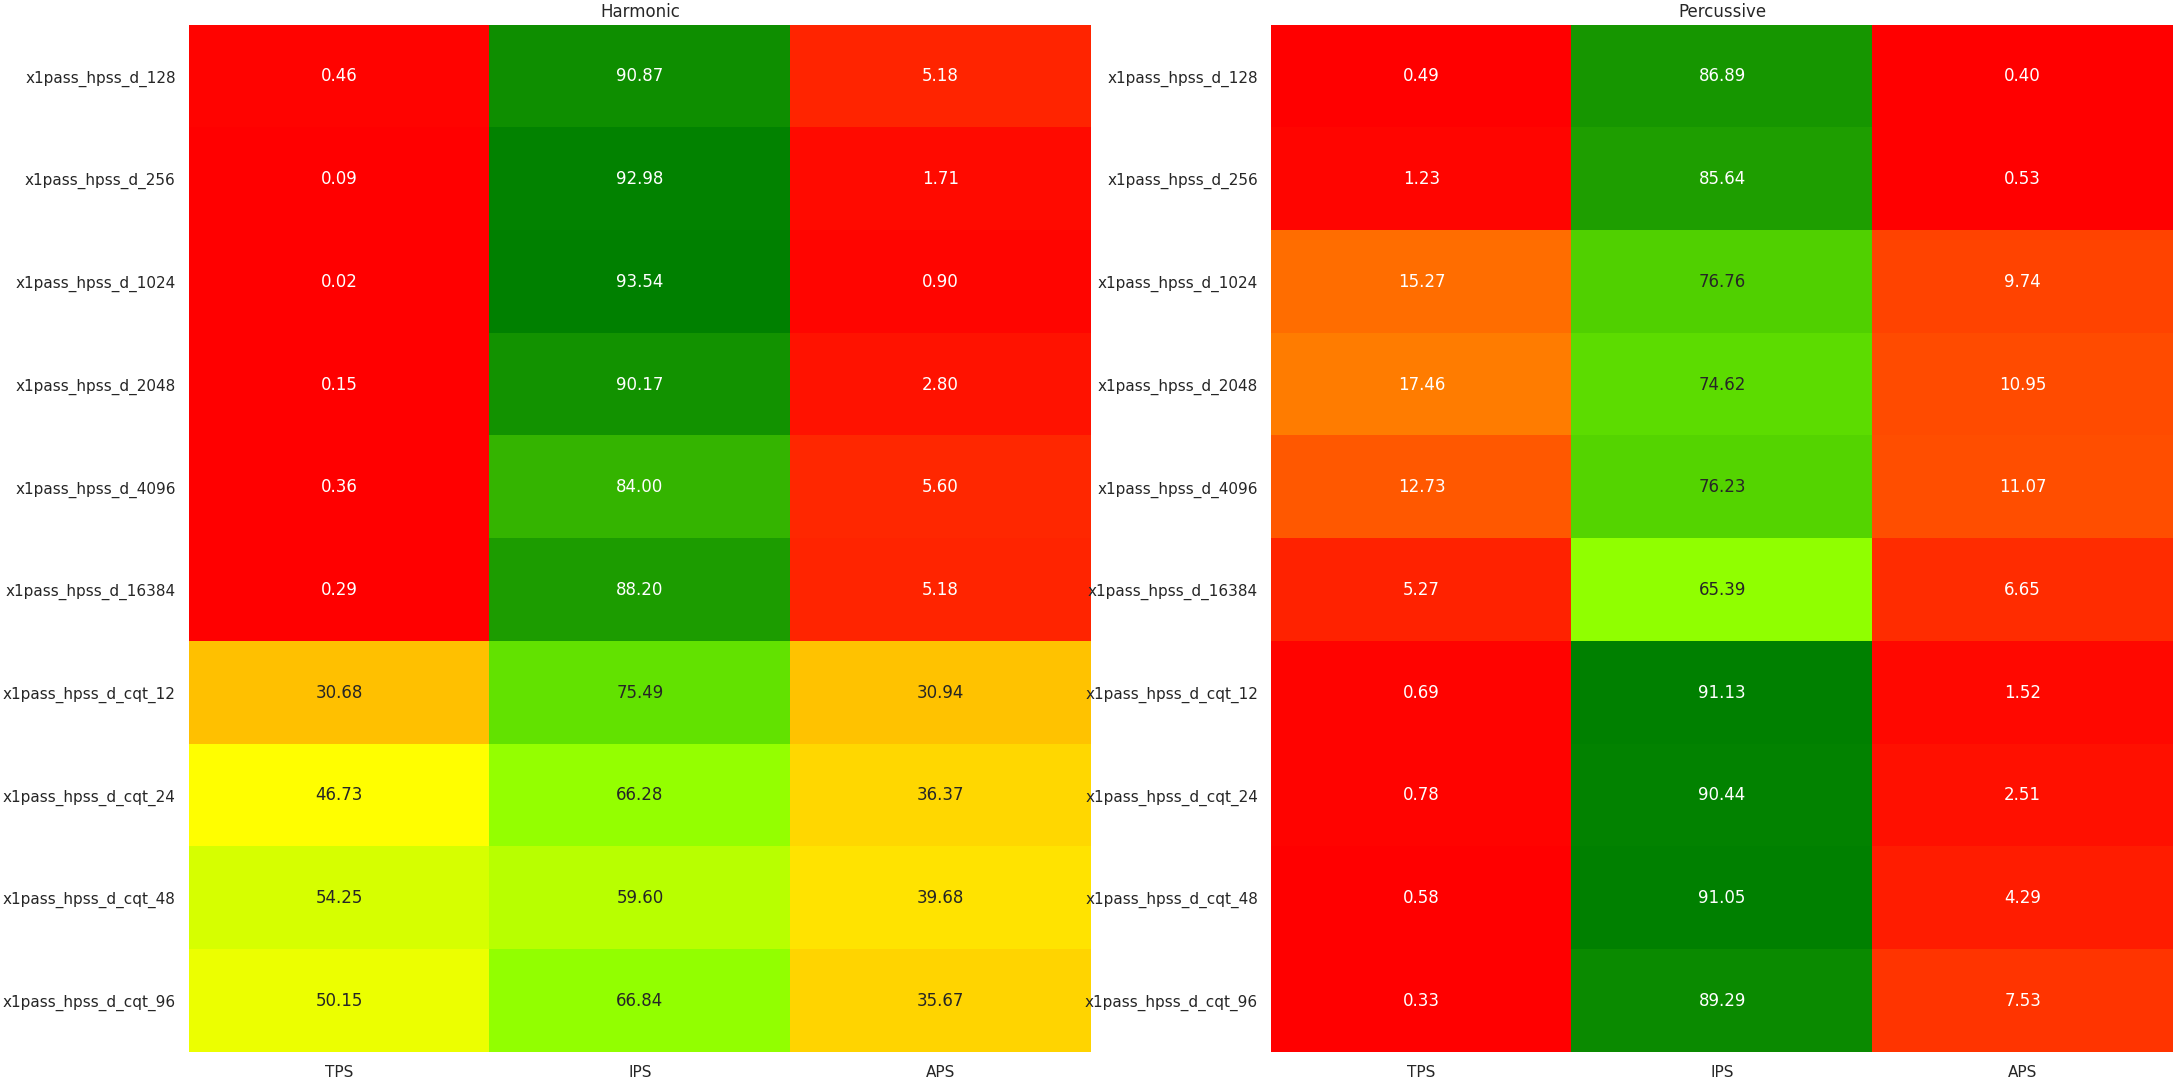
\includegraphics[width=16cm]{../evaluation/heatmaps/1pass_Driedger_PEASS_abbrev.png}}
	\caption{One-pass hard-masking PEASS results}
	\label{fig:round1hard}
\end{figure}

\vfill
\clearpage

\subsubsection{Realtime median-filtering}

In a previous project\footnote{\url{https://github.com/sevagh/Real-Time-HPSS}} presented for MUMT 501, the same 1-pass median filtering HPSS algorithms were adapted to work in realtime by using a sliding STFT and causal median filter. Figure \ref{fig:rthpss} describes the realtime system.

\begin{figure}[ht]
	\centering
	\subfloat[Sliding realtime STFT-ISTFT]{{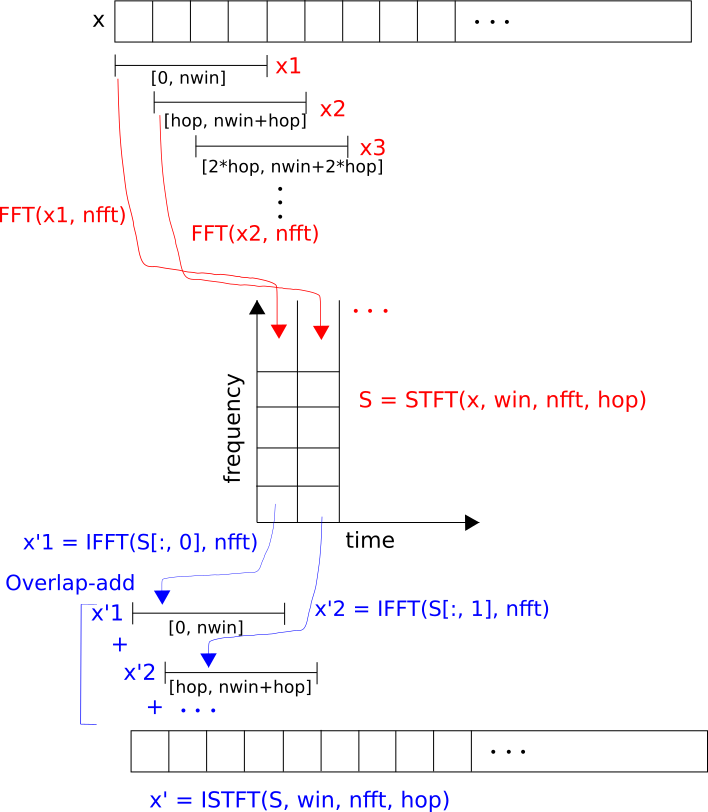
\includegraphics[height=8cm]{./slidingstft_diagram.png} }}
	\subfloat[Realtime HPSS block diagram]{{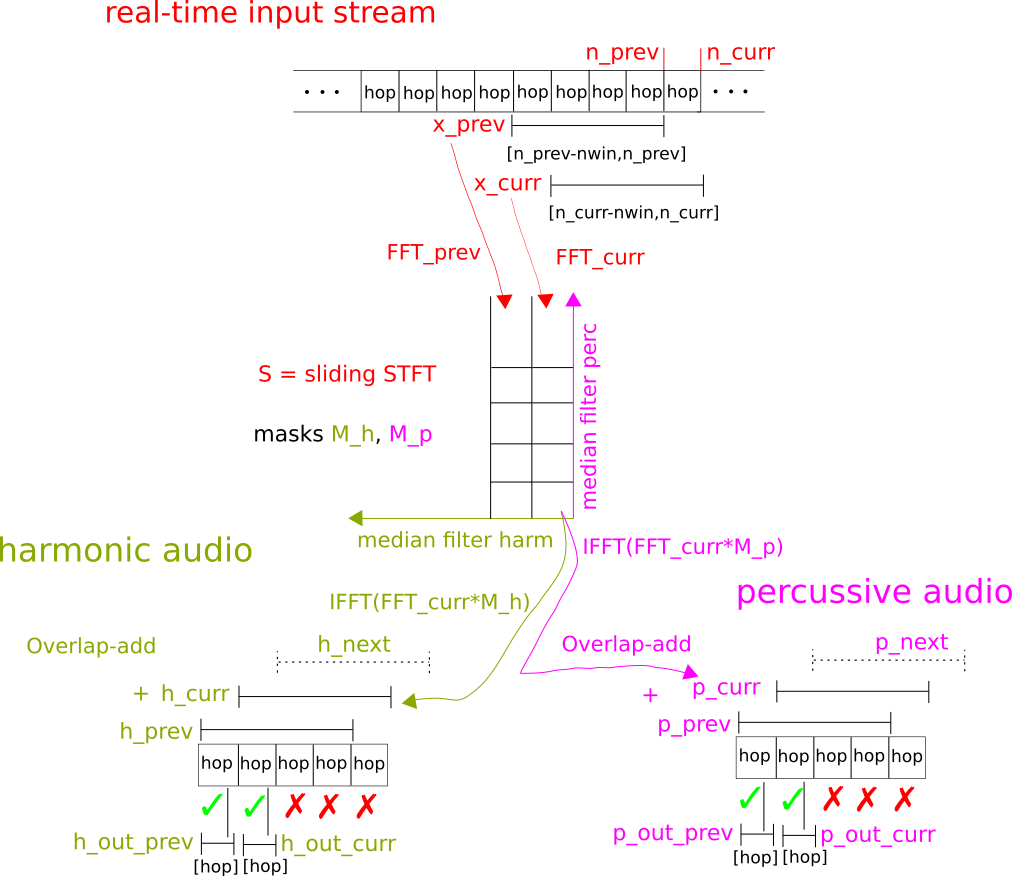
\includegraphics[height=8cm]{./rthpss_diagram.png} }}\\
	\vspace{0.1em}
	\subfloat[Realtime HPSS median filter causality]{{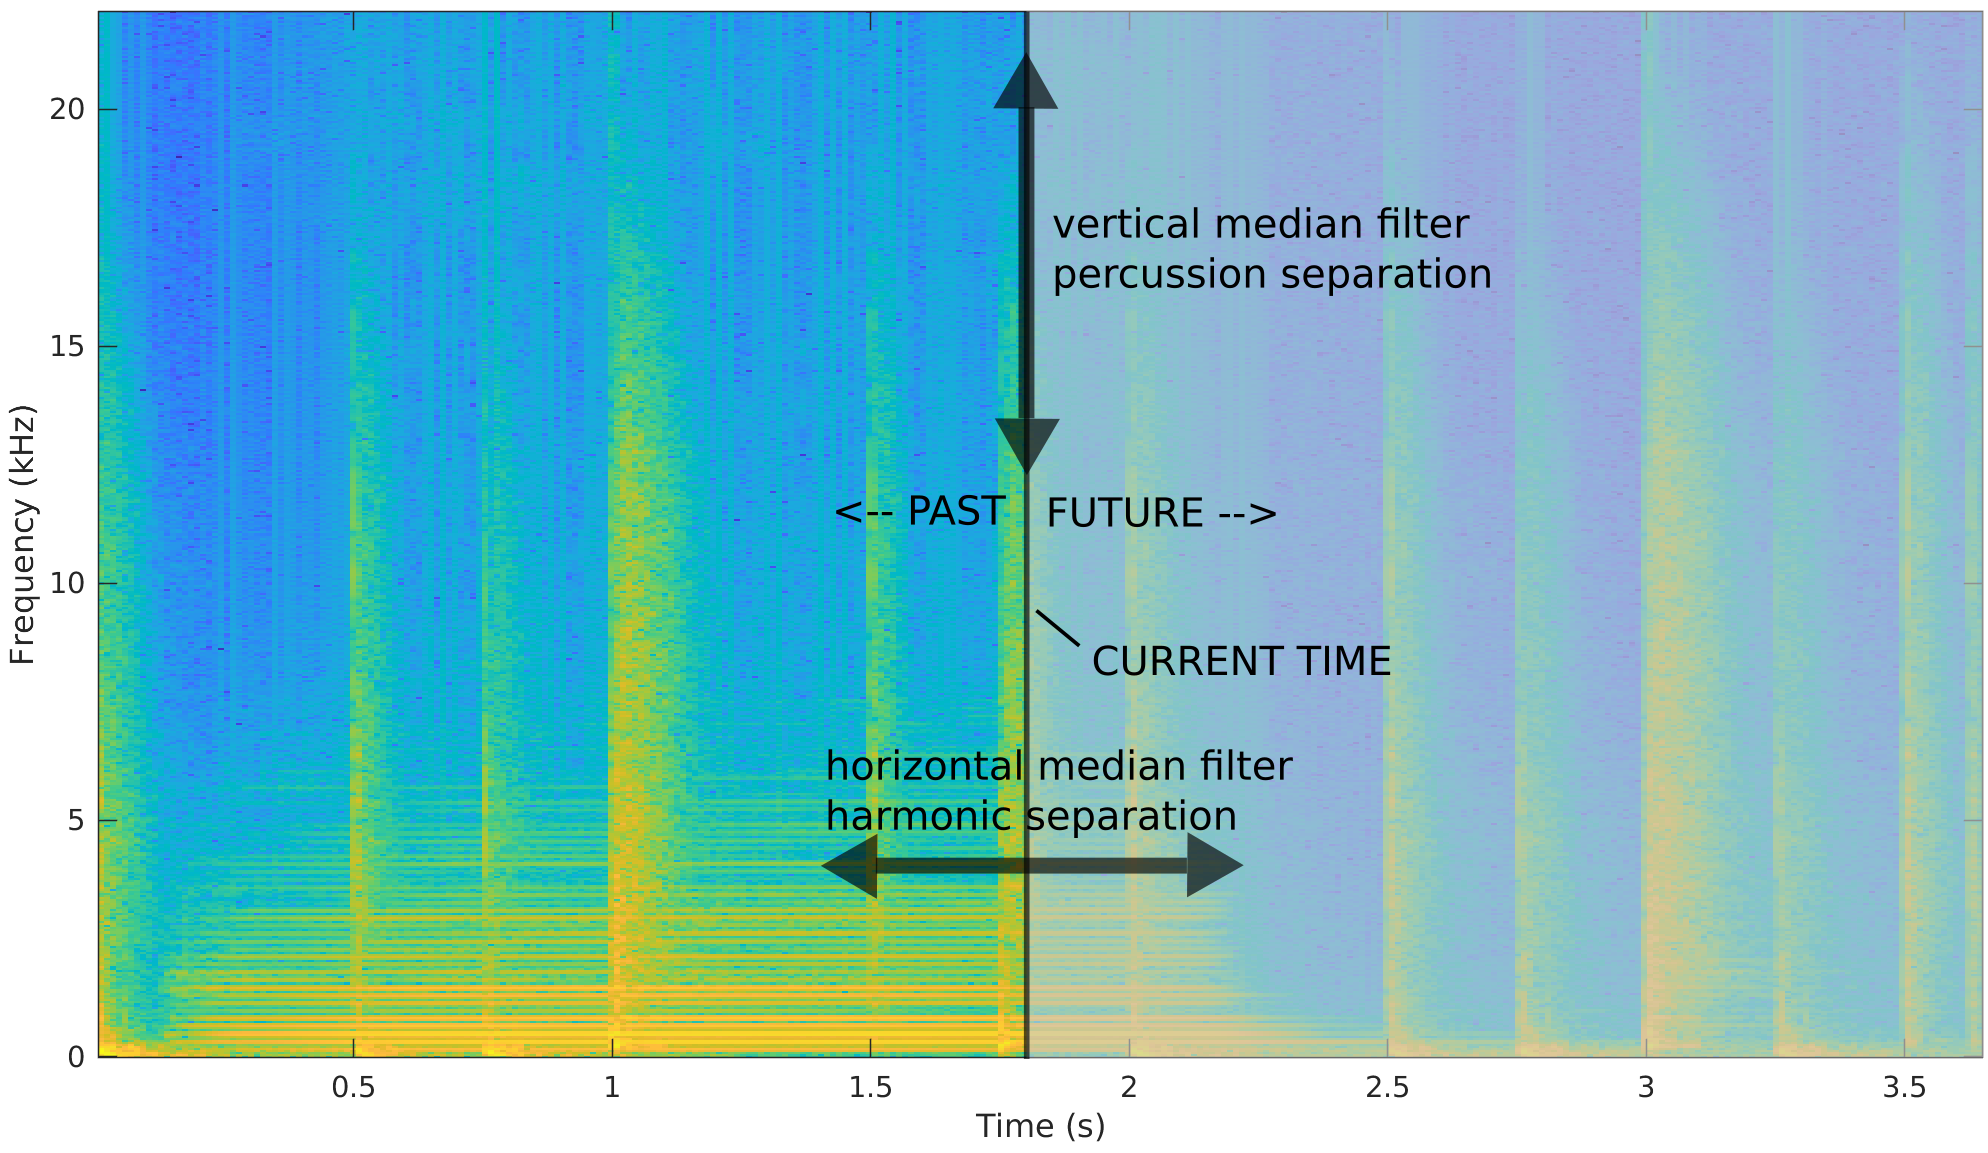
\includegraphics[height=6cm]{./rthpss_causality.png} }}
	\caption{Realtime median-filtering HPSS}
	\label{fig:rthpss}
\end{figure}

As shown in the results for the simple 1-pass median-filtering algorithms, the CQT with 96 bins per octave had a very good performance in harmonic and percussive separation when used in place of the linear-frequency STFT. The same idea is applied to the realtime STFT-based HPSS, to use the CQT. The realtime version of the CQT is the \textit{sliCQ transform}, or sliced constant-Q transform, described by \citet{rtcqt}. The implementation of realtime median filtering of the sliCQ transform was first attempted using the MATLAB implementation of sliCQ NSGToolbox,\footnote{\url{https://www.univie.ac.at/nonstatgab/toolbox.php}} but the code is not suitable for processing an input signal chunk-by-chunk (it takes the entire input signal). However, the officially recommended Python library for the NSGT\footnote{\url{https://github.com/grrrr/nsgt}} contains an implementation of sliCQ which accepts consecutive chunks of the signal.

In the realtime STFT, the hop size is set to be the same as the input stream size, and the window size is $2*\text{hop\_size}$. For example, for an input stream of 1024 samples per chunk, the hop between consecutive chunks is 1024, and every 2 consecutive hops from the stream are stored in a ringbuffer of size 2048 which is the windowed input to the STFT. The equivalent of hop in the sliCQ transform is the transition length, and the equivalent of the window size is the slice length. For a stream size of 1024, the transition length is therefore 1024, and the slice length is 4096.

One main difference between sliCQ and the NSGT-CQT is that sliCQ returns more than 1 channel of coefficients. If the CQT returns a square matrix of NxM, the sliCQ returns 3xNxM. However, as the median filter is a common operation for images which are typically multi-channel (3 channels for RGB, or 4 channels for RGBA), typical median filter functions (in MATLAB, scipy, etc.) can easily support higher dimensions of median filter. The typical 2D median filters for HPSS of dimensions $\text{L\_harmonic } \times 1$, $1 \times \text{L\_percussive}$ are simply extended to $1 \times \text{ L\_harmonic } \times 1$, $1 \times 1 \times \text{ L\_percussive}$, to operate across all 3 channels of the sliCQ transform coefficients. This is described visually in figure \ref{fig:3dmfilt}.

\begin{figure}[ht]
	\centering
	\includegraphics[width=14cm]{./3dmfilt.png}
	\caption{Graphic showing the 3D median filter for sliCQ coefficients}
	\label{fig:3dmfilt}
\end{figure}

One final issue is that with a small stream size of 1024 (which, at a 44100 Hz sample rate represents 23.2ms, reasonable as a realtime stream size), the input slice length of 4096 doesn't support as many frequency bins as we would prefer. The chosen scale was the octave scale with 12 bins per octave and frequency limits of 80Hz to 20000Hz.

In the previous project, the quality of the realtime separation was not analyzed. The same MATLAB code for Realtime-HPSS was reused in this project to take advantage of the MUSDB18-HQ/PEASS/BSSv4 testbench and evaluate the actual quality of the separation. Again, we benefit from the dual Python/MATLAB testbench by being able to compare the MATLAB implementation of Realtime-STFT-HPSS and the Python implementation of Realtime-sliCQ-HPSS. As these are both implemented in different languages, performing a latency or computation time comparison is not useful. The implementations should be considered as a concept or blueprint to test the idea of realtime HPSS, not a serious finished product.

The results for PEASS and BSSv4 are shown in figure \ref{fig:rtresults} with both the soft and hard masking strategies of \citet{fitzgerald1} and \citet{driedger} respectively. The stream size for both is set to 1024, implying a hop of 1024 and window of 2048 in the STFT, and a transition length of 1024 and slice length of 4096 in the sliCQ. The input wav files are processed one chunk at a time to simulate realtime stream processing.

The sliCQ HPSS with 12 bins per octave and hard masks performs the best, making it a good choice for realtime separation.

\begin{figure}[ht]
	\centering
	\makebox[\textwidth]{\includegraphics[width=16cm]{../evaluation/heatmaps/Realtime_PEASS_abbrev.png}}
	\vspace{1em}
	\makebox[\textwidth]{\includegraphics[width=16cm]{../evaluation/heatmaps/Realtime_BSSv4_abbrev.png}}
	\caption{Realtime HPSS results, PEASS and BSSv4 scores}
	\label{fig:rtresults}
\end{figure}

\vfill
\clearpage

\subsubsection{Two-pass algorithms with STFT/CQT masking}

\citet{driedger}'s iterative algorithm is presented for harmonic/percussive source separation. The algorithm is shown in listing \ref{lst:pseudocodes}. The conclusions from the previous round of testing are used to prepare 3 variants of two-pass hard masking HPSS:
\begin{tight_enumerate}
	\item
		The first variant, ``id'' (Iterative Driedger), uses an STFT-16384 in the first pass, and an STFT-2048 in the second pass (the best performing STFT configurations for harmonic and percussive separation, respectively).
	\item
		The second variant, ``id\_cqt1'' uses a CQT-96 in the first pass for the harmonic separation (top harmonic performer), and STFT-2048 (top percussive performer) in the second pass.
	\item
		The third variant, ``id\_default,'' is the default with the exact settings (STFT-4096 for harmonic, STFT-256 for percussive) from the paper \cite{driedger}.
\end{tight_enumerate}

The results in figure \ref{fig:round2hard} show that the CQT-96/STFT-2048 algorithm performs the best. By the PEASS evaluation, the target and artifact scores for the CQT-96/STFT-2048 variant are better, at the expense of a slightly lower interference score.

\begin{figure}[ht]
	\centering
	\makebox[\textwidth]{\includegraphics[width=14cm]{../evaluation/heatmaps/2pass_Driedger_PEASS_abbrev.png}}
	\caption{Two-pass hard-masking PEASS results}
	\label{fig:round2hard}
\end{figure}

\subsubsection{TFJigsaw}

An algorithm considered which uses a custom time-frequency analysis is the Time-Frequency Jigsaw Puzzle \cite{tfjigsaw}, implemented in LTFAT \cite{tfjigsaw2}. The implementation was adapted directly from the LTFAT demo \cite{tfjigsaw3}. Similar to the STFT or CQT algorithms above, the tfjigsawsep function in LTFAT allows for configuring the window size of the Gabor systems used for the tonal and transient components, which can be considered analogous to the two-pass methods seen above. The default settings are a Hann window of size 4096 for the tonal system and 256 for the transient system. The TFJigsaw algorithm is described in listing \ref{lst:tfjigsaw}.

\begin{figure}[h]
  \centering
  \centering
\begin{minted}[numbersep=\mintednumbersep,linenos,mathescape=true,breaklines,frame=single,escapeinside=||]{text}
|$f = \text{mixed audio}$|
|$a,M,\text{winsize},b\{1,2\} = \text{Gabor systems 1 and 2 configuration}$|
|$[\text{ref}1, \text{ref}2] = \text{generate estimate of random white noise entropy within supertile}$|
|$[\text{tau}1, \text{tau}2] = [\text{ref}1 \cdot r1, \text{ref}2 \cdot r2]$|
|$c1 = \text{DGTReal}(f, \text{winsize}1, a1, M1)\qquad\text{\textbf{Discrete Gabor Transform}}$|
|$c2 = \text{DGTReal}(f, \text{winsize}2, a2, M2)$|
|$f1 = \text{frequency supertile location, Gabor system 1}$|
|$f2 = \text{frequency supertile location, Gabor system 2}$|
|$t1 = \text{time supertile location, Gabor system 1}$|
|$t2 = \text{time supertile location, Gabor system 2}$|
|$[c1, c2] = \text{decision}(c1,c2,f1,f2,t1,t2,\text{tau}1,\text{tau}2)$|
|$f_{\text{tonal}} = \text{IDGTReal}(c1)\qquad\qquad\text{\textbf{Inverse discrete Gabor Transform}}$|
|$f_{\text{transient}} = \text{IDGTReal}(c2)$|
\end{minted}
  \captionof{listing}{TFJigsaw tonal/transient separation algorithm}
  \label{lst:tfjigsaw}
\end{figure}

The \Verb#decision# function uses R{\'e}nyi entropy to decide whether a signal is more random than random white noise represented within a supertile, and sets those coefficients to zero. For example, a transient sound will have a high entropy, or randomness, in the tonal Gabor system -- worse than white noise -- so it can be set to zero, creating a tonal separation (and vice-versa for transient separation). A consequence of using random white noise (in line 3 of the code listing) is that TFJigsawsep is non-deterministic. That is, you can run TFJigsaw separation with the same input signal and parameters, and get back a different result due to the different random white noise generated for the entropy comparison.

The parameters of Jigsaw Sep are as follows: $v2$ uses version 2 of the algorithm, $p$ is the proportion of the time-frequency supertile relative to the step sizes, $r1$ is the significance level of the tonal layer compared to white noise, and $r2$ is the same for the transient layer. General recommendations are $r2 > r1$, $r2 \approx 1.05$ for good percussion, $v2 = true$ for good tonal, $p = \text{small}$ for music separation. A variety of parameters were tested, shown in table \ref{table:round2jigsaw}.

\begin{table}[ht]
	\centering
\begin{tabular}{ |l|l|l|l|l|l|l|c|c|c|c|c|c|c| }
	 \hline
	  Name & p & r1 & r2 & v2 & winsize1 & winsize2 \\
	 \hline
	 \hline
	 tfjigsaw-1 & 2 & 0.88 & 1.05 & false & 4096 & 256 \\
	 \hline
	 tfjigsaw-2 & 2 & 0.88 & 1.05 & true & 4096 & 256 \\
	 \hline
	 tfjigsaw-3 & 4 & 0.88 & 1.05 & false & 4096 & 256 \\
	 \hline
	 tfjigsaw-4 & 2 & 0.88 & 1.03 & false & 4096 & 256 \\
	 \hline
	 tfjigsaw-5 & 2 & 0.85 & 1.05 & false & 4096 & 256 \\
	 \hline
	 tfjigsaw-6 & 2 & 0.88 & 0.89 & false & 4096 & 256 \\
	 \hline
	 tfjigsaw-7 & 2 & 0.85 & 1.05 & true & 4096 & 256 \\
	 \hline
	 tfjigsaw-8 & 5 & 0.85 & 1.05 & true & 4096 & 256 \\
	 \hline
	 tfjigsaw-9 & 9 & 0.85 & 1.05 & true & 4096 & 256 \\
	 \hline
	 tfjigsaw-10 & 2 & 0.88 & 1.03 & false & 16384 & 4096 \\
	 \hline
	 tfjigsaw-11 & 2 & 0.88 & 1.03 & false & 8192 & 2048 \\
	 \hline
	 tfjigsaw-12 & 2 & 0.85 & 1.05 & true & 16384 & 4096 \\
	 \hline
	 tfjigsaw-13 & 2 & 0.85 & 1.05 & false & 16384 & 4096 \\
	 \hline
	 tfjigsaw-14 & 2 & 0.88 & 1.05 & false & 16384 & 256 \\
	 \hline
	 tfjigsaw-15 & 2 & 0.88 & 1.05 & false & 16384 & 2048 \\
	 \hline
	 tfjigsaw-16 & 2 & 0.88 & 1.05 & false & 16384 & 1024 \\
	 \hline
	 tfjigsaw-17 & 2 & 0.88 & 1.05 & false & 8192 & 512 \\
	 \hline
\end{tabular}
	\caption{TFJigsaw configurations}
	\label{table:round2jigsaw}
\end{table}

From the tested configurations in figure \ref{fig:jigsaw}, we can see that the harmonic separation of configuration \Verb#tfjigsaw-1# achieves excellent results for target and artifacts -- it does not have the highest interference score, but this is usually a tradeoff, with better interference resulting from more aggressive removal, which results in more artifacts. In a subjective listening test, \Verb#tfjigsaw-1# sounds the best. On the other hand, good parameters could not be found for percussive separation scores for the TFJigsaw, which almost all suffered from a low artifact score (i.e., suffered from a presence of artifacts). This doesn't necessarily mean that TFJigsaw  is bad at percussive separation -- further study might be required to explore why this is the case, and how the results can be improved.

\begin{figure}[ht]
	\centering
	\makebox[\textwidth]{\includegraphics[width=16cm]{../evaluation/heatmaps/Jigsaw_PEASS_abbrev.png}}
	\makebox[\textwidth]{\includegraphics[width=16cm]{../evaluation/heatmaps/Jigsaw2_PEASS_abbrev.png}}
	\caption{TFJigsaw PEASS results}
	\label{fig:jigsaw}
\end{figure}

\vfill
\clearpage

\subsubsection{WMDCTLasso}

The last algorithm, WMDCTLasso\cite{wmdct}, also implemented in LTFAT \cite{wmdct3}. As seen before, there are two settings for window sizes of the Gabor systems used for the WMDCT frames used in the tonal and transient Gabor systems. The default settings are a Hann window of size 4096 for the tonal system and 256 for the transient system. The algorithm is described in listing \ref{lst:wmdctlasso}.

\begin{figure}[h]
  \centering
  \centering
\begin{minted}[numbersep=\mintednumbersep,linenos,mathescape=true,breaklines,frame=single,escapeinside=||]{text}
|$f = \text{mixed audio}$|
|$F1 = \text{frametight}(\text{frame}(\text{wmdct}, \text{gauss}, \text{winsize}_{h}))\qquad\text{\textbf{WMDCT frame transform} }$|
|$F2 = \text{frametight}(\text{frame}(\text{wmdct}, \text{gauss}, \text{winsize}_{p}))$|
|$c1 = \text{franagrouplasso}(F1, f, \lambda_{h}, \text{soft}, \text{freq})$|
|$c2 = \text{franagrouplasso}(F2, f, \lambda_{p}, \text{soft}, \text{time})$|
|$xh = \text{frsyn}(F1, c1)\qquad\qquad\qquad\text{\textbf{Inverse WMDCT frame transform} }$|
|$xp = \text{frsyn}(F2, c2)$|
\end{minted}
  \captionof{listing}{WMDCTLasso tonal/transient separation algorithm}
  \label{lst:wmdctlasso}
\end{figure}

The \Verb#franagrouplasso# function is provided in the LFAT, and solves the group lasso regression problem in the time-frequency domain. The theoretical background was covered in section \ref{sec:theorysparsity}. It is used in the WMDCTLasso algorithm to search for tonal components (with the `freq' argument), and transient components (with the `time' argument). The parameters of WMDCT are $\lambda$, or sparsity, for the Group Lasso regression for each of the tonal and transient systems, and Gaussian window sizes for the WMDCT frames for each system. A variety of parameter combinations were tested, shown in table \ref{table:round2wmdct}. The defaults, taken from the demo, are window sizes of 256 (tonal) and 32 (transient), and lambda values of 0.8 (tonal) and 0.5 (transient) for the percussive system.

\begin{table}[ht]
	\centering
\begin{tabular}{ |l|l|l|l|l|c|c|c|c|c| }
	 \hline
	  Name & $\lambda_{h}$ & $\lambda_{p}$ & $\text{winsize}_{h}$ & $\text{winsize}_{p}$ \\
	 \hline
	 \hline
	 wmdctlasso-1 & 0.8 & 0.5 & 256 & 32 \\
	 \hline
	 wmdctlasso-2 & 0.8 & 0.5 & 4096 & 64 \\
	 \hline
	 wmdctlasso-3 & 0.8 & 0.5 & 16384 & 128 \\
	 \hline
	 wmdctlasso-4 & 0.8 & 0.5 & 16384 & 256 \\
	 \hline
	 wmdctlasso-5 & 0.8 & 0.5 & 4096 & 256 \\
	 \hline
	 wmdctlasso-6 & 1.0 & 1.0 & 4096 & 64 \\
	 \hline
	 wmdctlasso-7 & 0.5 & 0.5 & 16384 & 128 \\
	 \hline
	 wmdctlasso-8 & 0.2 & 0.2 & 16384 & 256 \\
	 \hline
	 wmdctlasso-9 & 0.9 & 0.4 & 4096 & 256 \\
	 \hline
	 wmdctlasso-10 (same as 1) & & & & \\
	 \hline
	 wmdctlasso-11 & 0.8 & 0.5 & 512 & 32 \\
	 \hline
	 wmdctlasso-12 & 0.8 & 0.5 & 1024 & 32 \\
	 \hline
	 wmdctlasso-13 & 0.8 & 0.5 & 256 & 16 \\
	 \hline
	 wmdctlasso-14 & 0.8 & 0.5 & 256 & 8 \\
	 \hline
	 wmdctlasso-15 & 1.0 & 1.0 & 256 & 32 \\
	 \hline
	 wmdctlasso-16 & 0.2 & 0.5 & 256 & 32 \\
	 \hline
\end{tabular}
	\caption{WMDCT configurations}
	\label{table:round2wmdct}
\end{table}

From the tested configurations in figure \ref{fig:wmdct}, we can see results that look more like the hard-masking HPSS results (in figure \ref{fig:round1hard}). Interference is good, at the expense of artifacts, or artifacts and target are good, at the expense of interference. Another interesting effect of the WMDCLasso algorithm is that during the listening test, the effect on percussion sounded like a noise gate, with harmonic and vocals briefly being audible during a drum hit and then being strongly suppressed after. However, none of the tested configurations showed promising PEASS results, or good quality separation in the listening tests.

\begin{figure}[ht]
	\centering
	\makebox[\textwidth]{\includegraphics[width=16cm]{../evaluation/heatmaps/WMDCT2_PEASS_abbrev.png}}
	\makebox[\textwidth]{\includegraphics[width=16cm]{../evaluation/heatmaps/WMDCT_PEASS_abbrev.png}}
	\caption{WMDCT PEASS results}
	\label{fig:wmdct}
\end{figure}

\vfill
\clearpage

\subsubsection{Hybrid -- TFJigsaw-HPSS}

\begin{wrapfigure}{r}{5cm}
	\vspace{-1.0em}
	\includegraphics[width=5cm]{./hybrid_hpss_block_diagram.png}
	\caption{Hybrid HPSS}
	\label{fig:hybridhpss}
\end{wrapfigure}

The first hybrid algorithm created is for harmonic/percussive source separation. Noting that the \Verb#tfjigsaw-1# configuration achieved the best harmonic separation, and that median-filtering and soft masking with STFT-2048 achieved the best percussive separation, the proposed hybrid is a combination of both. First, the harmonic component is separated using TFJigsaw (the percussive output is discarded).

Next, median filtering with STFT-2048 is applied on the input signal, with a twist -- the percussive estimate is computed like typical, with a median filter. However, the harmonic estimate is computed by taking the STFT-2048 magnitude of the harmonic component output by TFJigsaw. The harmonic estimate from median filtering the STFT is discarded.

Finally, soft masks are computed from the percussive and harmonic estimates and applied to the STFT to get the percussive component. The block diagram of the proposed system is presented in figure \ref{fig:hybridhpss}.

In figure \ref{fig:finalhpss}, we can see that the hybrid HPSS combines good harmonic and percussive separations from the two original algorithms, respectively. The PEASS scores show that it compares favorably with the Open-Unmix neural network solution. The vocal hybrid (which will be shown next) has better percussive separation performance across all scores, but slightly worse interference in the harmonic separation.

\begin{figure}[ht]
	\centering
	\makebox[\textwidth]{\includegraphics[width=16cm]{../evaluation/heatmaps/Final_HPSS_PEASS_abbrev.png}}
	\caption{Final HPSS results, PEASS scores}
	\label{fig:finalhpss}
\end{figure}

\subsection{Harmonic/percussive/vocal source separation}

The next task is harmonic/percussive/vocal source separation. The mixtures are combined from the instrument stems including vocals from the same 5 minutes of MUSDB18-HQ, and as before, the PEASS results are shown in heatmaps.

\subsubsection{Median-filtering with STFT/CQT masking}
\label{subsec:mfvocalsep}

The median filtering algorithms and a general framework for two-pass median filtering harmonic/percussive source separation were provided in \ref{subsec:mfilthpss}. The paper \cite{fitzgerald2} noted the following:
\begin{tight_enumerate}
	\item
		Using an STFT-16384 in the first pass led to a good harmonic separation
	\item
		Using an STFT-1024 in the second pass led to a good percussive separation
	\item
		Using a CQT-24 in the second pass led to a good vocal separation
\end{tight_enumerate}

The results are shown in figure \ref{fig:vocalround1soft}, and the algorithm names and configurations are described in table \ref{table:round3softvocal}. One interesting outcome is that using a CQT-96 in the first iteration in place of the STFT-16384 resulted in a better vocal and percussive separation, at the expense of the harmonic separation. The paper's original results were reproduced -- the variant with two linear STFTs (STFT-16384, STFT-1024) produced a better percussive and worse vocal separation, and the variant with a linear STFT and nonlinear CQT (STFT-16384, CQT-24) produced a better vocal separation.

\begin{table}[ht]
	\centering
\begin{tabular}{ |l|l|l|c|c|c| }
	 \hline
	  Name & First pass & Second pass  \\
	 \hline
	 \hline
	 mf\_default\_linear & STFT-16384 & STFT-1024 \\
	 \hline
	 mf\_default\_cqt & STFT-16384 & CQT-24 \\
	 \hline
	 mf\_cqt1 & CQT-96 & STFT-1024 \\
	 \hline
	 mf\_cqt2\_\{12-96\} & STFT-16384 & CQT-\{12-96\} \\
	 \hline
	 mf\_cqt3\_\{12-96\} & CQT-96 & CQT-\{12-96\} \\
	 \hline
\end{tabular}
	\caption{Multipass Fitzgerald configurations}
	\label{table:round3softvocal}
\end{table}

The vocal separation has a stable quality in every case where the second pass is a CQT, regardless of the values for bins-per-octave. The percussive separation is best with a linear STFT-1024 in the second pass, but respectable with the CQT up to 48 bins-per-octave.

When choosing between the harmonic separation scores of the linear STFT-16384 and nonlinear CQT-96 in the first pass, we can see that using a CQT gives a very high target and artifact score, but a very poor interference score. In other words, there is hardly any separation being done. On the other hand, the target score of STFT-16384's harmonic separation is very low, indicating the absence of the desired sound.

\vfill
\clearpage % force a page break before references

\subsubsection{Hybrid -- Iterative-CQT-Sep}

\begin{wrapfigure}{r}{8cm}
	\includegraphics[width=8cm]{./hybrid_vocal_block_diagram.png}
	\caption{Hybrid harmonic/percussive/vocal block diagram}
	\label{fig:hybridvocal}
\end{wrapfigure}

In section \ref{subsec:mfvocalsep}, \citet{fitzgerald2}'s multipass algorithm for harmonic/percussive/source separation was presented and evaluated. The authors' findings were confirmed -- following a first iteration for harmonic separation with an STFT-16384, using a CQT-24 in the second iteration gives a good vocal estimate, and using an STFT-1024 in the second gives a good percussive estimate. It was also noted that using the CQT-96 in the first iteration led to a higher quality percussive or vocal separation in the next iteration, but created a high-interference harmonic separation. The hybrid combines all of the above findings with some refinements:

\begin{tight_enumerate}
	\item
		Median-filter CQT-96 in the first position -- the harmonic output is the ``almost final'' harmonic component, and the percussive output is the next input.
	\item
		Median-filter CQT-24 in the second iteration, where the harmonic output is the final vocal component. Add the percussive separation from this iteration to the percussive output of previous iteration, to use as the next input.
	\item
		Median-filter STFT-1024 in the third, where the percussive output is the final percussive component.
	\item
		Using a CQT-12, get harmonic, vocal, and percussive magnitude estimates from the ``almost final'' harmonic and final vocal and percussive components. Create and apply a soft mask for harmonic refinement, in an attempt to reduce vocal and percussive interference.
\end{tight_enumerate}

The system is shown in the block diagram in figure \ref{fig:hybridvocal}. The results of the evaluation are in figure \ref{fig:finalvocal}. The hybrid vocal algorithm gets the best percussive score, beating the multipass Fitzgerald configuration from the paper\cite{fitzgerald2} which had the highest percussive score. The harmonic score sacrifices interference for a better target and artifact scores. However, note that the interference score (16.32) is higher than the original interference score of the CQT-96 in the first position (4.81). This shows that the fourth step for harmonic refinement had the desired effect of reducing the interference in the harmonic separation.

\begin{figure}[ht]
	\centering
	\makebox[\textwidth]{\includegraphics[width=16cm]{../evaluation/heatmaps/2pass_Fitzgerald_PEASS_abbrev.png}}
	\caption{Multipass Fitzgerald (soft mask) PEASS results}
	\label{fig:vocalround1soft}
	\vspace{1em}
	\makebox[\textwidth]{\includegraphics[width=16cm]{../evaluation/heatmaps/Final_Vocal_PEASS_abbrev.png}}
	\caption{Final vocal results, PEASS scores}
	\label{fig:finalvocal}
\end{figure}

\vfill
\clearpage % force a page break before references

\section{Discussion and conclusion}

It is important to mention that despite showing good PEASS scores, a conclusion cannot be made that the presented hybrid algorithms beat Open-Unmix. Open-Unmix claims state-of-the-art results \cite{umxsota} in the BSS metric. In the SigSep community, the BSS evaluation measure used is BSSv4, their own modification, available in their Python libraries museval\cite{museval} and bsseval\cite{bsseval}.

To avoid questions of bias, evaluations on the final HPSS and vocal algorithms were redone using the bsseval library, containing SigSep's own BSSv4 implementation. Based on the modular Python and MATLAB testbench in this project, it was simple to write a new Python script which traverses the previous separation directory and computes BSSv4 metrics and heatmaps. The BSSv4 metrics can be seen in figures \ref{fig:bssv4hpss} and \ref{fig:bssv4vocal}.

Although the hybrids are no longer shown to beat Open-Unmix, some previous conclusions based on the PEASS scores are also observed with the BSSv4 scores:

\begin{tight_itemize}
	\item
		In the HPSS task, the 1-pass soft mask algorithm using a single CQT-96 shows a strong harmonic and percussive separation performance in BSSv4, confirming that it is a good choice for a simple and low-cost implementation. However, it still suffers from a low interference score in the harmonic component. It has very good percussive performance, beating both hybrids.
	\item
		In the HPSS task, both hybrids have a better target and artifact score than the original iterative Driedger algorithm, although worse interference -- again, consistent with the expectations from soft and hard TF masking \cite{masking}.
	\item
		In the harmonic/percussive/vocal separation task, the hybrid-vocal algorithm has a better interference score than mf-cqt1 (which uses a CQT-96 in the first iteration's harmonic separation). This confirms that step 4 of the hybrid vocal algorithm, the harmonic refinement step, achieves the desired effect of boosting the interference-related score (at the expense of a lower target score).
	\item
		In the harmonic/percussive/vocal separation task, both original configurations of \citet{fitzgerald2} are beat by the hybrid-vocal in the target and artifact score of all 3 components (harmonic, percussive, and vocal). However, the original configurations have a better interference score.
\end{tight_itemize}

In contemporary source separation literature\cite{nussl}, \citet{fitzgerald1}'s original HPSS algorithm is referred to as primitive. In SiSEC 2018\cite{sigsep2018}, HPSS scored very low in the evaluations, and the evaluation campaign revealed that deep learning solutions are getting the best results for source separation. This report showed that by considering different aspects of time-frequency resolution, respectable results could be obtained while maintaining the simplicity of the original median-filtering idea. Using a CQT with 96 bins-per-octave in place of the STFT gives surprisingly good performance in harmonic/percussive source separation, and creating a multi-iteration hybrid algorithm with multiple CQTs (and one STFT), still only using simple median-filtering and soft masking, led to strong separation results for harmonic/percussive/vocal components.

While the PEASS scores make the median-filtering based techniques look promising, the situation is not as clear-cut when considering BSSv4 scores. For this, I have opened a GitHub issue with the SigSep community,\footnote{\url{https://github.com/sigsep/sigsep-mus-eval/issues/78}} discussing how I found unexpected results in the PEASS scores, and asking if they have considered PEASS over BSS when designing or evaluating Open-Unmix.

\begin{figure}[ht]
	\centering
	\makebox[\textwidth]{\includegraphics[width=16cm]{../evaluation/heatmaps/Final_HPSS_BSSv4_abbrev.png}}
	\caption{Final HPSS results, BSSv4 scores}
	\label{fig:bssv4hpss}
	\vspace{1em}
	\makebox[\textwidth]{\includegraphics[width=16cm]{../evaluation/heatmaps/Final_Vocal_BSSv4_abbrev.png}}
	\caption{Final vocal results, BSSv4 scores}
	\label{fig:bssv4vocal}
\end{figure}

\vfill
\clearpage % force a page break before references

%\nocite{*}
\section{References}
\printbibliography[heading=none]

\vfill
\clearpage %force a page break

\begin{appendices}

\section{\textbf{\textcolor{red}{TODO }}Code and results}

\end{appendices}

\end{document}
